\documentclass[11pt,a4paper]{article}

% ---------------------------------------------------------------------------
% Packages (matched to the existing sibling reports in reports/)
% ---------------------------------------------------------------------------
\usepackage[T1]{fontenc}
\usepackage[utf8]{inputenc}
\usepackage[htt]{hyphenat}
\setlength{\emergencystretch}{3em}
\usepackage[a4paper,margin=2.4cm]{geometry}
\usepackage{graphicx}
\usepackage{subcaption}
\usepackage{booktabs}
\usepackage{longtable}
\usepackage{tabularx}
\usepackage{array}
\usepackage{enumitem}
\usepackage{caption}
\usepackage{float}
\usepackage{xcolor}
\usepackage[hidelinks]{hyperref}
\usepackage{url}

\graphicspath{{figures/}}
\captionsetup{font=small,labelfont=bf}
\setlist{topsep=2pt,itemsep=1pt,parsep=0pt}
\newcolumntype{L}[1]{>{\raggedright\arraybackslash}p{#1}}
\newcommand{\code}[1]{\texttt{#1}}

\title{\textbf{Code Report}\\[0.4em]
\large Software Implementation of a Governed Multi-Agent System for\\
Autonomous E-Commerce and Accounting Operations}
\author{Research Engineer / Software Architect\\\small Governed Multi-Agent AI for Autonomous E-Commerce and Accounting Operations}
\date{\today}

\begin{document}

% ===========================================================================
% TITLE PAGE
% ===========================================================================
\begin{titlepage}
\centering
\vspace*{1.2cm}
{\Huge\bfseries Code Report\par}
\vspace{0.5cm}
{\Large Software Implementation of a Governed Multi-Agent System for\\[2pt]
Autonomous E-Commerce and Accounting Operations\par}
\vspace{1.0cm}
{\large An evidence-based description of the source code, its architecture,\\
its execution paths, its tests and its implementation gaps\par}
\vspace{1.6cm}
\vfill
{\small
\begin{tabular}{rl}
\textbf{Document type:} & Software implementation (code) report \\[4pt]
\textbf{Scope:} & Repository \code{MultiAgentAI-Research} at the time of inspection \\[4pt]
\textbf{Code inspected:} & \code{reports/dataset\_report/analysis/}, \\
 & \code{reports/dataset\_report/tests/}, \\
 & \code{reports/dataset\_selection\_table/scripts/}, \\
 & \code{reports/Agents reports/figures/} \\[4pt]
\textbf{Companion reports:} & \code{reports/dataset\_selection\_table/main.tex} \\
 & (project/dataset overview), \\
 & \code{reports/dataset\_report/dataset\_report.tex} (Dataset Report), \\
 & \code{reports/Agents reports/Agent\_Report.tex} (Agent Report) \\[4pt]
\textbf{Diagrams:} & \code{figures/} (generated by \code{figures/make\_figures.py}) \\[4pt]
\textbf{Date:} & \today \\
\end{tabular}
}
\vfill
{\small\itshape Integrity note. This report documents only what exists in the repository. Inspection found \textbf{no agent implementation}: all seven conceptual agents are recorded as \emph{designed but not implemented}, and the only executable software is a dataset analysis, validation and reporting pipeline. Every implementation claim below is supported by a file path, a symbol name or a measured command output. Where a step could not be verified, this is stated explicitly.}
\end{titlepage}

% ===========================================================================
% ABSTRACT
% ===========================================================================
\begin{abstract}
\noindent
This report documents the software that actually exists in the repository of the research project \emph{Governed Multi-Agent AI for Autonomous E-Commerce and Accounting Operations}. Repository inspection found \textbf{2{,}144 lines of Python across eleven files, containing 65 functions and zero classes}, plus three LaTeX report sources. There is \textbf{no agent implementation, no orchestration layer, no message schema, no policy engine and no audit store}; the directory \code{src/} is empty and the root \code{README.md} is a zero-byte file. The implemented software is (i) a reproducible dataset-analysis and validation package under \code{reports/dataset\_report/analysis/} with seven modules and a \code{python -m analysis} entry point, which reads both raw datasets read-only and writes 26 CSV files, one JSON summary and thirteen figures; (ii) an independent, standard-library dataset inspector under \code{reports/dataset\_selection\_table/scripts/inspect\_datasets.py}; and (iii) two figure-generation scripts for the sibling reports. The analysis package is covered by thirteen unit tests, all of which were executed for this report and pass (\code{13 passed in 1.49\,s}), and the full pipeline was re-executed and verified to be deterministic: all 27 generated files were reproduced with byte-identical SHA-256 digests. Inspection also produced three concrete, verified defects: a mis-detected CSV dialect in the inspector that over-counts the Olist review table by 26 rows, an empty \code{src/} placeholder, and the complete absence of a dependency manifest. Each of the seven conceptual agents is assessed individually and assigned the status \emph{designed but not implemented}; where the data layer already computes a relevant primitive (for example the payment-versus-item reconciliation proxy, or IQR outlier fences) this is stated precisely and is not presented as an agent. No performance figure, no fraud-detection result and no capability is fabricated. A prioritized roadmap converts the current pipeline into a stable ingestion and validation layer on which the agents can be built.
\end{abstract}

\tableofcontents
\clearpage

% ===========================================================================
% GLOSSARY
% ===========================================================================
\section*{Glossary, Abbreviations and Status Vocabulary}
\addcontentsline{toc}{section}{Glossary, Abbreviations and Status Vocabulary}
\begin{tabularx}{\textwidth}{L{3.2cm}X}
\toprule
\textbf{Term} & \textbf{Meaning in this report} \\ \midrule
Agent & A software component with an explicit role, inputs, outputs and a governance-wrapped interface. \\ 
Audit event & A record of an action and its decision context. \textbf{No audit event is produced by the current code.} \\ 
BRL & Brazilian Real, the currency implied by the Olist marketplace context. \\ 
Entry point & A module that can be started directly: \code{python -m analysis} or \code{python .../inspect\_datasets.py}. \\ 
Gate & A validation check that raises on failure and therefore aborts the run (fail-closed). \\ 
GBP & Pound sterling, the currency of Online Retail II. \\ 
Inspector & The standard-library script \code{inspect\_datasets.py} in \code{reports/dataset\_selection\_table/scripts/}. \\ 
Provenance manifest & The SHA-256-per-file listing written to \code{dataset\_inventory.csv}. It is \emph{not} an audit trail. \\ 
Implemented & Present as executable code, evidenced by a file path and a symbol name. \\ 
Partially implemented & Implemented in a narrow form, with a named limitation; never described as complete. \\ 
Designed but not implemented & Specified in the sibling reports or in qualitative CSV columns, but with no executable code. \\ 
Not found in repository & No design and no code; used only where the design also does not exist. \\ 
\bottomrule
\end{tabularx}

% ===========================================================================
\section{Executive Summary}
% ===========================================================================
\paragraph{Software objective.} The codebase is intended to become the executable substrate of a governed multi-agent system \cite{wooldridge2009,shoham2009,russellNorvig2021} that coordinates e-commerce operations, inventory analysis, accounting tasks, anomaly detection, governance enforcement and audit traceability. At present the codebase implements the \emph{front} of that system: a reproducible pipeline that ingests the two research datasets, validates their structure, profiles them, derives a small set of defensible aggregate facts, and exports machine-readable and human-readable evidence for the sibling reports.

\paragraph{What kind of system the repository contains.} Inspection is unambiguous: the repository contains a \textbf{dataset analysis and validation pipeline together with a documentation and reporting pipeline}. It does \emph{not} contain a working multi-agent system, nor even a partial prototype of one. There are no agent classes --- in fact there are no class definitions anywhere in the repository --- no orchestrator, no message bus, no policy engine and no audit store. The directory \code{src/} exists but is empty, and the root \code{README.md} is empty. Consequently all seven conceptual agents are classified as \emph{designed but not implemented} (Section~\ref{sec:agents}).

\paragraph{Main implemented modules.} The substantive implementation is the Python package \code{reports/dataset\_report/analysis/}, comprising \code{config}, \code{profiling}, \code{olist}, \code{online\_retail}, \code{compare}, \code{figures} and the \code{\_\_main\_\_} entry point. A second, independent program, \code{reports/dataset\_selection\_table/scripts/inspect\_datasets.py}, performs a standard-library inventory and quality scan of the same raw files, and \code{reports/Agents reports/figures/make\_figures.py} renders the schematic diagrams of the Agent Report. Table~\ref{tab:inventory} quantifies all Python in the repository.

\paragraph{Technologies.} Python 3.10.11 \cite{pythonDocs} with pandas 2.3.3 \cite{mckinney2010,pandasDocs}, NumPy 1.26.4 \cite{harris2020numpy,numpyDocs}, matplotlib 3.10.7 \cite{hunter2007matplotlib,matplotlibDocs}, seaborn 0.13.2 \cite{waskom2021seaborn,seabornDocs}, openpyxl 3.1.5 \cite{openpyxlDocs} and pytest 9.1.0 \cite{pytestDocs}, plus the Python standard library; MiKTeX-pdfTeX 4.18 with BibTeX 4.1 \cite{miktexDocs} for the LaTeX reports (Section~\ref{sec:env}). No LLM framework, no agent-orchestration library, no machine-learning library, no API client and no database driver are used.

\paragraph{Implementation maturity.} The data layer is mature enough to be trustworthy: it is deterministic, it fails closed on two structural violations, it is unit-tested at the helper level, and its thirteen tests pass. The agent layer has zero maturity: nothing exists. Governance is enforced only to the extent that the data layer validates columns and timestamps; no authorization, policy decision, approval or audit event exists.

\paragraph{Principal limitations.} (i) The seven agents, orchestration, governance enforcement and audit are absent. (ii) There is no dependency manifest, so the environment is not pinned. (iii) The inspector contains a verified CSV-dialect defect that over-counts the Olist review table by 26 rows (99{,}250 instead of 99{,}224), which propagates into the dataset-selection artifacts and into \code{main.tex}. (iv) The code has no logging, no output validation, no CLI for the analysis package, and no integration or end-to-end tests. These are documented with evidence in Section~\ref{sec:limits}.

% ===========================================================================
\section{Introduction and Software Scope}
\label{sec:scope}
% ===========================================================================
\subsection{Role of the codebase in the research project}
The research project studies how governed, specialised software agents can cooperate on e-commerce and accounting workflows while remaining traceable, a design-science undertaking in the sense of Hevner et al.~\cite{hevner2004}. Four artefacts support that study: the project/dataset overview (delivered as \code{reports/dataset\_selection\_table/main.tex}; no file named literally \code{Main\_Report} exists in the repository), the Dataset Report (\code{reports/dataset\_report/dataset\_report.tex}), the Agent Report (\code{reports/Agents reports/Agent\_Report.tex}), and this Code Report. This document is the only one that concentrates on \emph{software}: how the code is organised, what it executes, how data flows through it, how it is tested, and what remains to be built. Dataset statistics are therefore not repeated here; the reader is referred to the Dataset Report \cite{olistDataset,chen2012}. Agent responsibilities, the governance lifecycle and the proposed data contracts are not repeated either; the reader is referred to the Agent Report.

\subsection{Concept, proposal, implementation and plan}
The task distinguishes four things, and this report keeps them separate at all times.
\begin{itemize}
\item \textbf{Research concept.} A governed multi-agent system for autonomous e-commerce and accounting operations, with seven agent roles (Section~\ref{sec:agents}).
\item \textbf{Proposed architecture.} The layered design, the governance lifecycle, the audit event schema and the evaluation protocol specified in the sibling reports. These are \emph{design documents}, not code.
\item \textbf{Implemented software.} The dataset analysis and validation package, the stdlib inspector and the figure generators, all listed in Table~\ref{tab:repo} and analysed in Section~\ref{sec:code}.
\item \textbf{Planned features.} The roadmap of Section~\ref{sec:roadmap}.
\end{itemize}

\subsection{What the current code can actually execute}
Running the code today performs exactly four operations, all verified during preparation of this report:
\begin{enumerate}
\item \code{python -m analysis} (from \code{reports/dataset\_report}) reads the nine Olist CSV files and both Online Retail II worksheets read-only, computes profiling, key, referential-integrity, join, distribution, temporal and monetary metrics, derives a payment-versus-item reconciliation proxy and several retail business signals, writes 26 CSV files and one JSON summary into \code{analysis\_results/}, and renders thirteen PNG figures into \code{figures/}.
\item \code{python reports/dataset\_selection\_table/scripts/inspect\_datasets.py} (from the repository root) performs an independent, standard-library inventory and quality scan and writes five CSV artifacts plus an \code{inspection\_summary.json}.
\item \code{python figures/make\_figures.py} (in \code{reports/Agents reports/figures} or in \code{reports/code\_report/figures}) renders schematic diagrams for the respective report.
\item \code{python -m pytest tests -q} (from \code{reports/dataset\_report}) executes thirteen unit tests.
\end{enumerate}
Nothing in the repository accepts a business request, plans a task, selects an agent, evaluates a policy, requests approval or records an audit event. Those operations are not implemented in any form.

% ===========================================================================
\section{Development Environment and Technologies}
\label{sec:env}
% ===========================================================================
The environment was characterised by direct runtime inspection rather than by reading a manifest, because \textbf{no dependency manifest exists}: there is no \code{requirements.txt}, \code{environment.yml}, \code{pyproject.toml}, \code{setup.py}, \code{Pipfile} or lock file anywhere in the repository. Versions below were obtained with \code{python --version}, \code{pip list}, \code{pytest --version} and \code{pdflatex --version} in the working environment, and cross-checked against imports actually present in the source and against the compiled byte-code file names (for example \code{test\_analysis.cpython-310-pytest-9.1.0.pyc}). Where a version could not be established this is stated.

\begin{table}[H]
\centering
\small
\begin{tabularx}{\textwidth}{L{3.1cm}L{2.5cm}L{4.2cm}X}
\toprule
\textbf{Technology} & \textbf{Version} & \textbf{Purpose in this repository} & \textbf{Evidence in repository} \\
\midrule
Python & 3.10.11 & Language runtime for all code & \code{python --version}; byte-code names \code{*.cpython-310*.pyc} in \code{analysis/\_\_pycache\_\_} and \code{tests/\_\_pycache\_\_} \\
pandas & 2.3.3 & CSV/Excel loading, profiling, joins, aggregation & \code{import pandas as pd} in \code{analysis/config.py}, \code{profiling.py}, \code{olist.py}, \code{online\_retail.py}, \code{\_\_main\_\_}; \code{pip list} \\
NumPy & 1.26.4 & numeric dtypes, quantiles, IQR fences, NaN handling & \code{import numpy as np} in \code{profiling.py}, \code{olist.py}, \code{online\_retail.py}, \code{figures.py} \\
matplotlib & 3.10.7 & figure rendering (Agg backend) & \code{matplotlib.use("Agg")} in \code{analysis/figures.py} and \code{figures/make\_figures.py} \\
seaborn & 0.13.2 & plot theme and statistical plots & \code{import seaborn as sns} in \code{analysis/figures.py} \\
openpyxl & 3.1.5 & Excel engine for \code{pandas.read\_excel} & \code{engine="openpyxl"} in \code{online\_retail.load\_sheets()} \\
pytest & 9.1.0 & unit-test runner & \code{tests/test\_analysis.py}; \code{pytest --version}; \code{*.pytest-9.1.0.pyc} \\
Python standard library & 3.10.11 & inspector, hashing, I/O helpers & \code{csv}, \code{zipfile}, \code{xml.etree.ElementTree}, \code{hashlib}, \code{argparse}, \code{json}, \code{pathlib} in \code{inspect\_datasets.py} and \code{config.py} \\
\LaTeX{} (MiKTeX-pdfTeX) & 4.18 (MiKTeX 24.1) & compilation of report sources & \code{pdflatex --version}; \code{*.tex} and \code{*.pdf} in \code{reports/} \\
BibTeX & 4.1 (MiKTeX 24.1) & bibliography processing & \code{bibtex --version}; \code{references.bib} and \code{*.bbl} in \code{reports/} \\
\bottomrule
\end{tabularx}
\caption{Technologies verified to be used by the repository's code, with the file evidence. No library is listed merely because it is common in AI projects.}
\label{tab:tech}
\end{table}

\paragraph{Technologies deliberately absent.} The following were checked and are \textbf{not used}: LLM and agent frameworks (no \code{langchain}, \code{langgraph}, \code{autogen}, \code{crewai}, \code{openai} or \code{anthropic} import exists, and none is installed); machine-learning or anomaly-detection libraries (no \code{scikit-learn}); API/client libraries; database drivers; web frameworks; workflow engines; task queues; and configuration/secrets managers. Packages such as \code{pydantic} 2.13.4 and \code{scipy} 1.15.3 are present in the working environment but are imported by no repository file, so they are not project dependencies either. This absence is the single most important environmental fact for this report: there is no infrastructure in which an agent could run.

\paragraph{Operating-system assumptions.} All code is platform-independent Python. Two practical Windows observations apply: the sibling READMEs document commands for Windows PowerShell, and one path containing a space (\code{reports/Agents reports/}) must be quoted on any command line. The analysis package derives all paths from \code{\_\_file\_\_}, so it does not depend on the current working directory beyond the requirement to run it as a module from \code{reports/dataset\_report} (Section~\ref{sec:exec}).

% ===========================================================================
\section{Repository Structure}
\label{sec:repo}
% ===========================================================================
Table~\ref{tab:repo} describes every relevant file and directory. Generated caches, byte-code directories and the raw datasets themselves are excluded from the table and, in the case of the raw files, are described under ``External data''.

\begin{table}[H]
\centering
\footnotesize
\begin{tabularx}{\textwidth}{L{4.6cm}L{5.3cm}L{2.4cm}L{2.1cm}}
\toprule
\textbf{File or directory} & \textbf{Responsibility} & \textbf{Main dependencies} & \textbf{Status} \\
\midrule
\code{README.md} & None; file is empty (0 bytes) & --- & Empty \\
\code{src/} & Intended source root; \textbf{empty directory} & --- & Placeholder \\
\code{datasets/olist/} & Nine Olist CSV tables (read-only input) & --- & External data \\
\code{datasets/\allowbreak online\_retail\_ii/\allowbreak online\_retail\_II.xlsx} & Two-worksheet Excel workbook (read-only input) & --- & External data \\
\code{reports/\allowbreak dataset\_report/\allowbreak analysis/\allowbreak config.py} & Paths, file hashing, deterministic writers & \code{hashlib}, \code{json}, \code{pathlib}, pandas & Implemented \\
\code{.../analysis/profiling.py} & Seven dataset-agnostic profiling helpers & pandas, NumPy & Implemented \\
\code{.../analysis/olist.py} & Olist loading, schema validation, key/RI/join/monetary analysis & pandas, NumPy, \code{config}, \code{profiling} & Implemented \\
\code{.../analysis/online\_retail.py} & Excel loading, cleaning, quality and business-signal metrics & pandas, NumPy, \code{config}, \code{profiling} & Implemented \\
\code{.../analysis/compare.py} & Inventory, comparative table, agent-suitability matrix & pandas, \code{config} & Implemented (mixed measured + curated text) \\
\code{.../analysis/figures.py} & Thirteen analysis figures & matplotlib, seaborn, \code{config} & Implemented \\
\code{.../analysis/\_\_main\_\_.py} & Entry point \code{main()}; orchestration of the pipeline & all of the above & Implemented \\
\code{.../analysis/\_\_init\_\_.py} & Package docstring and \code{\_\_all\_\_} & --- & Implemented \\
\code{.../tests/test\_analysis.py} & Thirteen unit tests of helper definitions & pytest, NumPy, pandas & Implemented \\
\code{.../analysis\_results/} & 26 CSV artifacts + \code{summary.json} & generated by \code{analysis} & Generated artifact \\
\code{.../figures/} & Thirteen PNG analysis figures & generated by \code{analysis} & Generated artifact \\
\code{reports/\allowbreak dataset\_report/\allowbreak dataset\_report.tex/.pdf} & Dataset Report (companion) & \LaTeX{} & Documentation \\
\code{reports/\allowbreak dataset\_selection\_table/\allowbreak scripts/inspect\_datasets.py} & Independent stdlib inventory and quality scanner & stdlib only & Implemented \\
\code{reports/\allowbreak dataset\_selection\_table/\allowbreak main.tex/.pdf} & Project and dataset overview (companion; no \code{Main\_Report} file exists) & \LaTeX{} & Documentation \\
\code{reports/\allowbreak dataset\_selection\_table/\allowbreak *.csv, inspection\_summary.json} & Inspector artifacts & generated & Generated artifact \\
\code{reports/\allowbreak Agents reports/\allowbreak Agent\_Report.tex/.pdf} & Agent design and implementation-status report & \LaTeX{} & Documentation \\
\code{reports/\allowbreak Agents reports/\allowbreak figures/make\_figures.py} & Seven schematic PNGs for the Agent Report & matplotlib & Implemented \\
\bottomrule
\end{tabularx}
\caption{Relevant repository contents and their status. Byte-code caches, \code{.pytest\_cache} directories and the large raw data files are omitted. \textbf{Bold} entries indicate findings that matter for the roadmap.}
\label{tab:repo}
\end{table}

\paragraph{Not present.} There is no \code{requirements.txt}, \code{pyproject.toml}, \code{setup.py}, skill file, container definition, Makefile, \code{tox.ini}, \code{pytest.ini}, \code{conftest.py}, CI workflow, \code{.gitignore}, database schema, API module, agent module, prompt file, model configuration, or secrets file. A targeted search for credential-like identifiers (API keys, tokens, passwords) found no configuration or secret material in the repository; the only pattern matches were ordinary Portuguese words inside Olist customer-review text files. No credentials therefore need to be, or can be, reported.

% ===========================================================================
\section{Software Architecture}
\label{sec:arch}
% ===========================================================================
The implemented architecture is a single-process, offline, batch pipeline. Figure~\ref{fig:repo} shows the actual module relationships and simultaneously marks the proposed components that have no implementation.

\begin{figure}[H]\centering
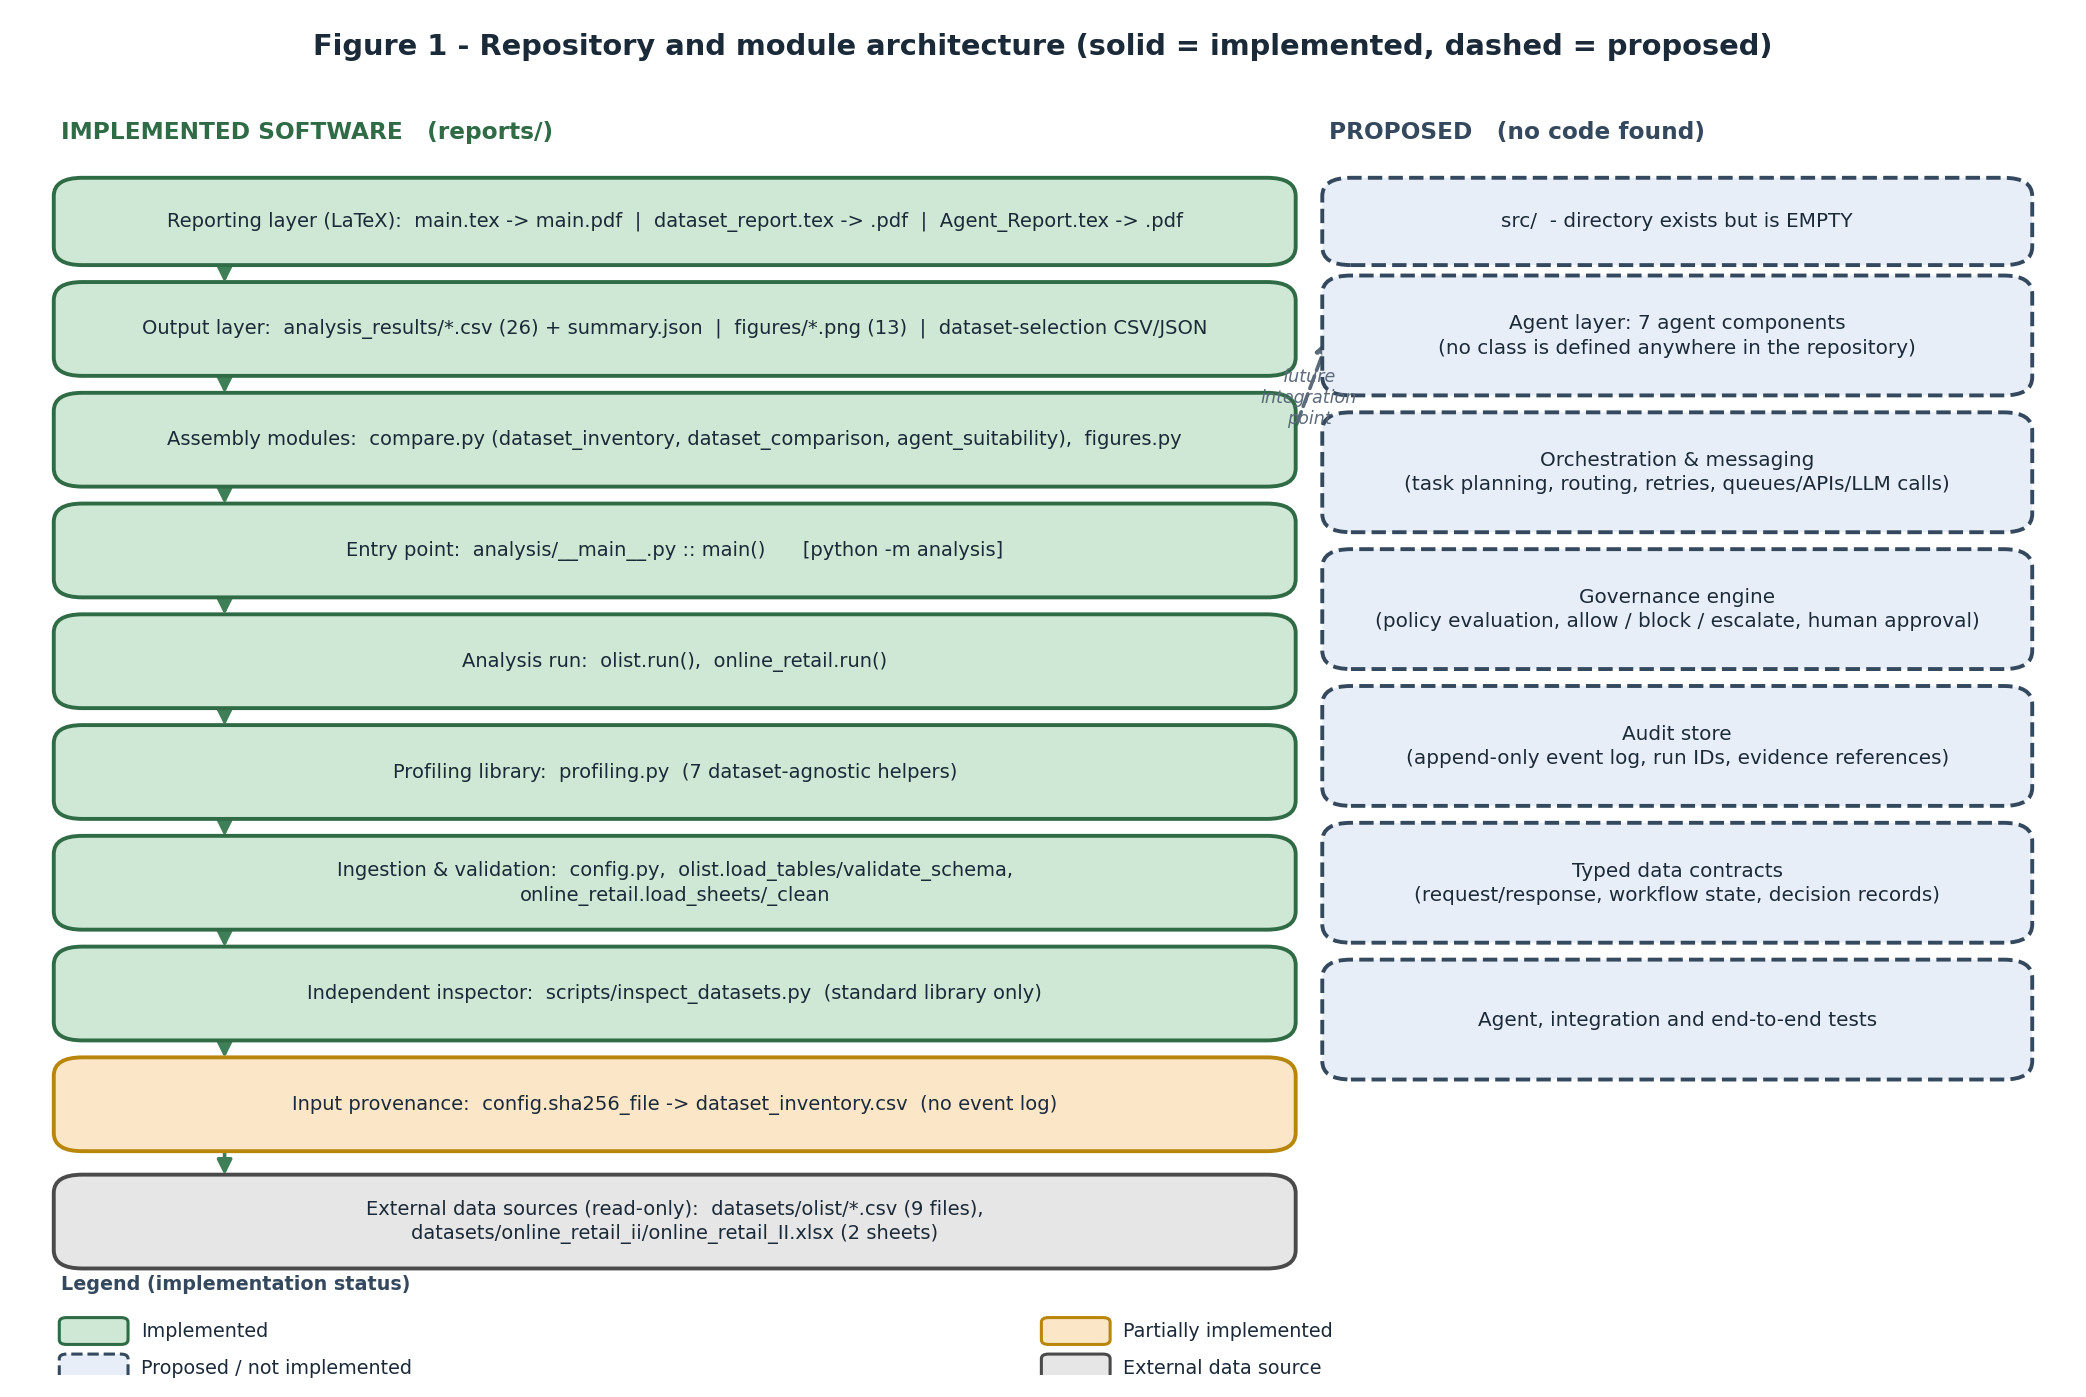
\includegraphics[width=\textwidth]{fig_repo_architecture.png}
\caption{Repository and module architecture as observed. Green solid boxes are implemented code; amber marks the partially implemented provenance mechanism; dashed boxes are proposed and have no implementation in the repository; grey marks external read-only data.}
\label{fig:repo}
\end{figure}

\subsection{Layer by layer}
\begin{itemize}
\item \textbf{Application entry point.} \code{analysis/\_\_main\_\_.py}, function \code{main()}, executed as \code{python -m analysis} from \code{reports/dataset\_report}. It calls every other module in a fixed order and is the only orchestrator that exists. The inspector has its own \code{main()} reached through \code{argparse}.
\item \textbf{Configuration layer.} \code{analysis/config.py} derives \code{REPO\_ROOT}, \code{OLIST\_DIR}, \code{RETAIL\_XLSX}, \code{RESULTS\_DIR} and \code{FIGURES\_DIR} from \code{\_\_file\_\_}, declares the input inventory (\code{OLIST\_FILES}, \code{RETAIL\_SHEETS}, \code{OLIST\_TABLE\_ORDER}) and provides \code{ensure\_dirs()}, \code{sha256\_file()}, \code{write\_csv()}, \code{write\_json()} and \code{round\_pct()}.
\item \textbf{Data access layer.} \code{olist.load\_tables()} (\code{pd.read\_csv}) and \code{online\_retail.load\_sheets()} (\code{pd.read\_excel}) are the only readers. Both are strictly read-only. The inspector implements its own readers, including a pure-Python OOXML reader \code{xlsx\_rows()}.
\item \textbf{Validation layer.} \code{olist.validate\_schema()} compares column \emph{sets} against \code{EXPECTED\_COLUMNS}; \code{olist.load\_tables()} aborts if timestamp parsing would create new \code{NaT}; \code{online\_retail.\_clean()} aborts unless the sheet columns equal \code{EXPECTED\_COLS} exactly. These are the only enforced gates in the repository.
\item \textbf{Processing and analysis layer.} \code{profiling.py} supplies seven reusable helpers; \code{olist.run()} and \code{online\_retail.run()} compose them with dataset-specific key, referential-integrity, join, distribution, temporal, monetary and business-signal logic.
\item \textbf{Agent layer.} \textbf{Not implemented.} No class exists anywhere in the repository; \code{src/} is empty.
\item \textbf{Orchestration layer.} \textbf{Not implemented} beyond the linear sequence inside \code{main()}. There is no task decomposition, routing, dependency resolution, retry or consolidation.
\item \textbf{Governance layer.} \textbf{Not implemented.} Column and type validation exist but are data-quality controls, not policy enforcement: there is no authorization step, no policy rule set, no allow/block/escalate decision and no approval gate.
\item \textbf{Audit and logging layer.} \textbf{Not implemented}, except for one partial primitive: \code{config.sha256\_file()} records a SHA-256 digest per source file into \code{dataset\_inventory.csv}, which is an input-integrity manifest. There is no event log, no run identifier, no actor, no decision record and no persistence layer. The Python \code{logging} module is never imported; progress is written with \code{print()}.
\item \textbf{API or user interface layer.} \textbf{Not implemented.} The only interface is the command line plus the generated PDF reports.
\item \textbf{Output and reporting layer.} Implemented: \code{config.write\_csv()}, \code{config.write\_json()}, \code{figures.py} and \code{compare.py} produce the artifacts consumed by the LaTeX sources.
\end{itemize}

\subsection{Architectural character}
The design is a strict batch DAG executed in a fixed order with no branching in the happy path: load $\rightarrow$ validate $\rightarrow$ profile $\rightarrow$ analyse $\rightarrow$ serialise $\rightarrow$ plot. Data crosses module boundaries as plain \code{dict}s of \texttt{pandas} \code{DataFrame}s (the \code{frames}/\code{facts} convention). There is no asynchronous behaviour, no concurrency, no persistence beyond file writes and no external service interaction. The architecture is appropriate for its current purpose (reproducible dataset analysis) and is, by construction, the opposite of what a multi-agent system requires.

% ===========================================================================
\section{Main Execution Workflow}
\label{sec:workflow}
% ===========================================================================
There are three execution paths. Figure~\ref{fig:workflow} shows all three, including the two fail-closed gates.

\begin{figure}[H]\centering
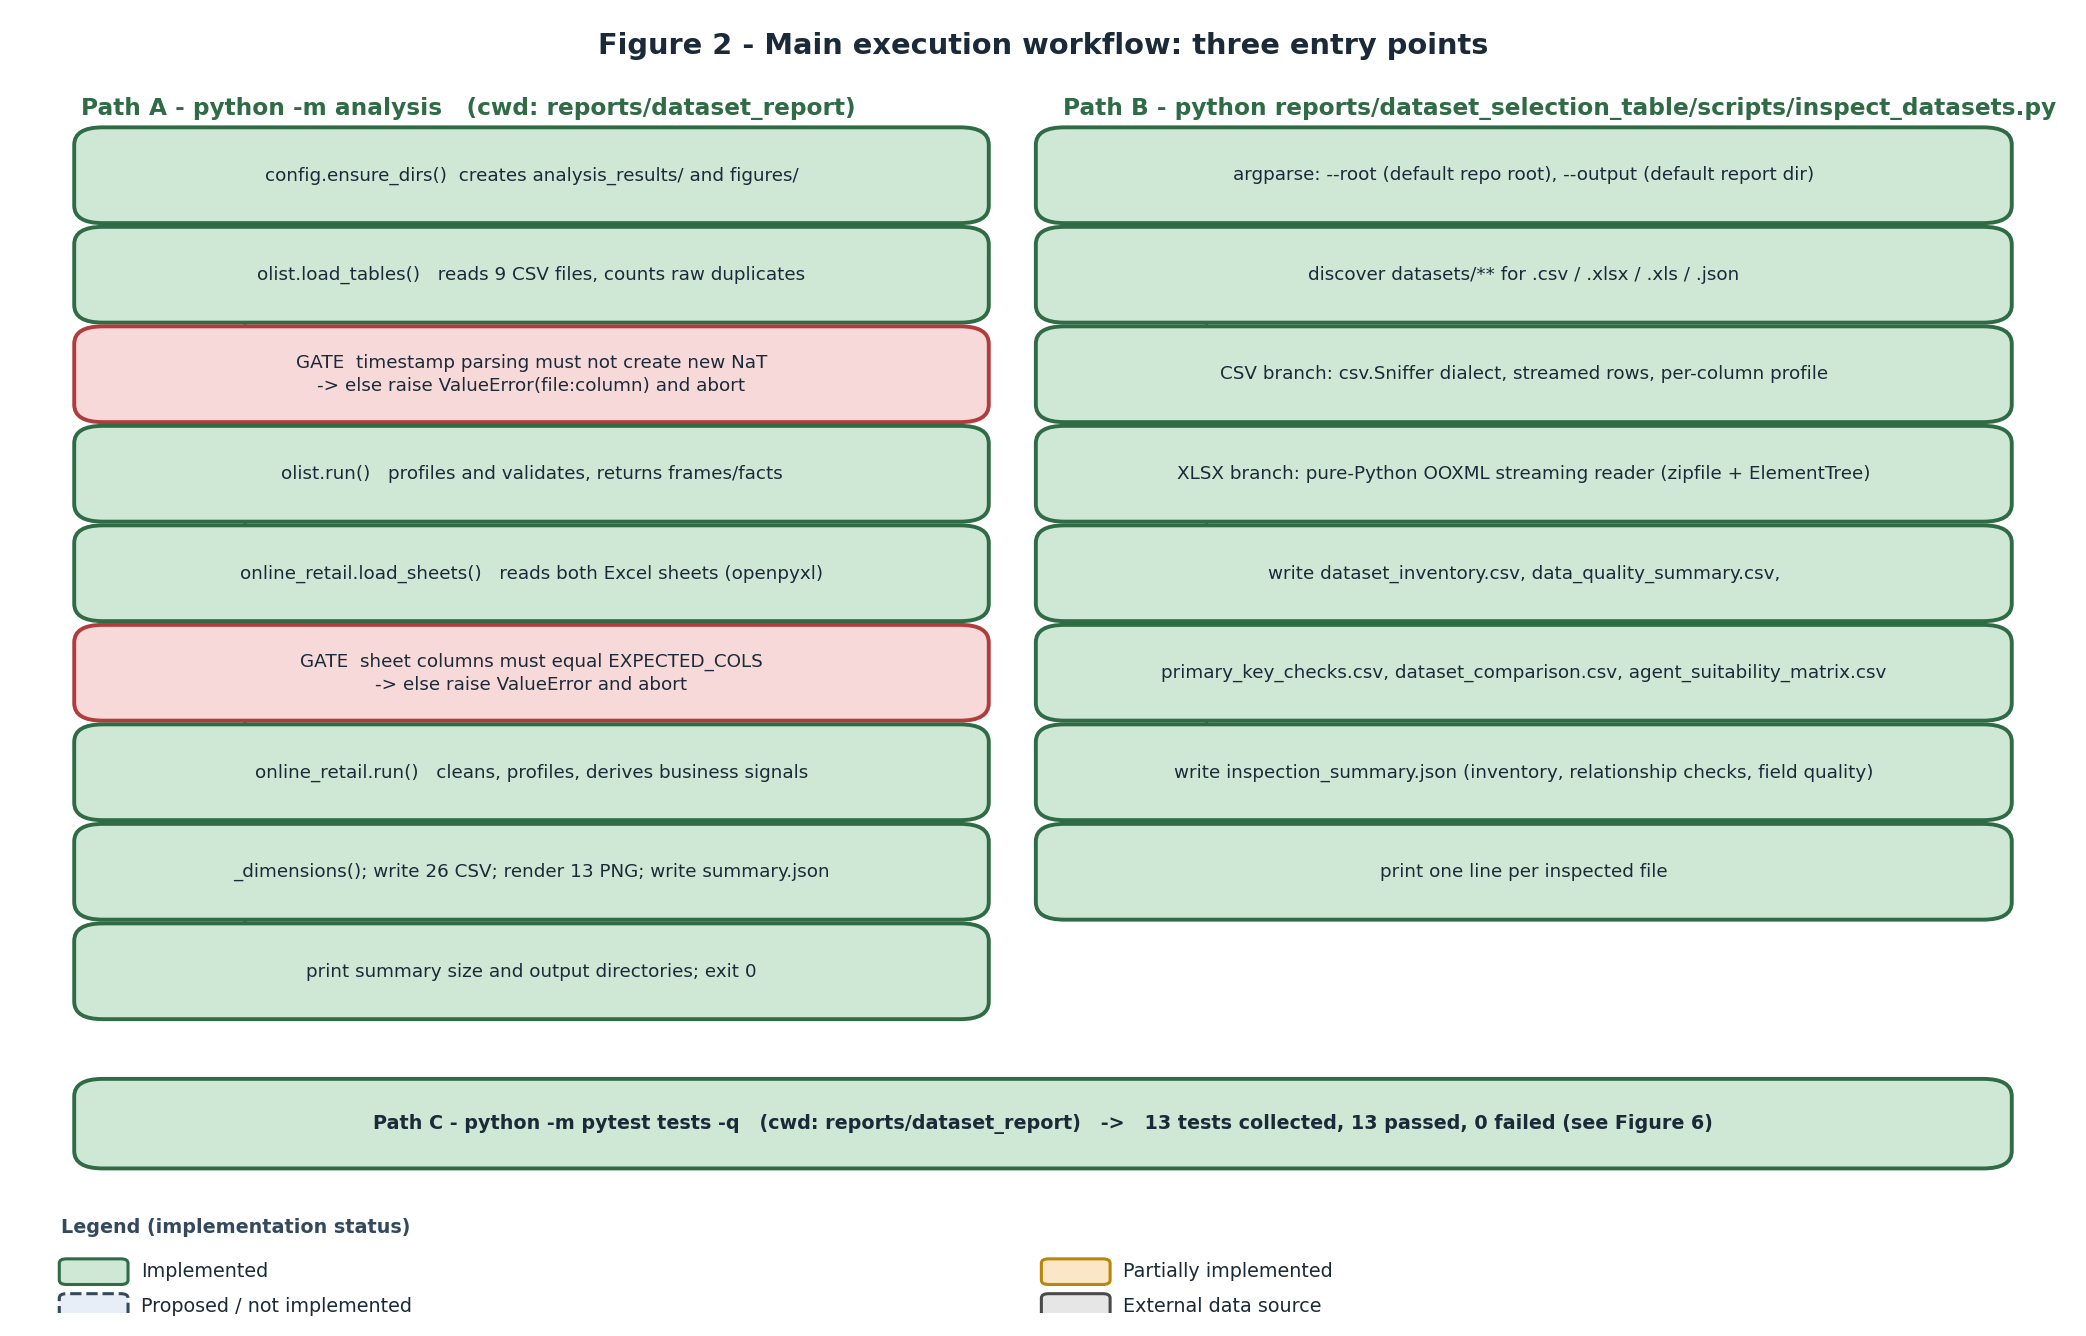
\includegraphics[width=\textwidth]{fig_execution_workflow.png}
\caption{The three real execution paths. Path~A is the analysis package, Path~B the standard-library inspector, Path~C the test suite. Amber boxes are validation gates that raise and abort the run.}
\label{fig:workflow}
\end{figure}

\subsection{Path A --- \code{python -m analysis}}
\begin{enumerate}
\item \textbf{Start.} The interpreter imports the package \code{analysis} and executes \code{analysis/\_\_main\_\_.py}.
\item \textbf{Configuration.} \code{config.ensure\_dirs()} creates \code{analysis\_results/} and \code{figures/} if absent. All other configuration is compile-time constants in \code{config.py}; nothing is read from the environment or a file.
\item \textbf{Input selection.} \code{olist.load\_tables()} iterates the fixed list \code{config.OLIST\_FILES}; \code{online\_retail.load\_sheets()} reads all sheets of \code{config.RETAIL\_XLSX}. There is no argument to select or filter inputs.
\item \textbf{Validation and processing.} For each Olist table the loader counts exact-duplicate rows on the raw values, then parses the columns named in \code{DATE\_COLUMNS} and \emph{raises} if parsing would turn a previously present value into \code{NaT}. \code{olist.run()} then validates the schema, profiles every table, and runs key checks, referential-integrity checks, join-cardinality and join-inflation measurements, distributions, temporal-integrity checks, monetary summaries and the payment-versus-item reconciliation proxy. For the workbook, \code{online\_retail.\_clean()} enforces the exact column list and then normalises codes, strings, dates and numerics, preserving genuine missing values as \code{pd.NA}.
\item \textbf{Invocation of components.} All invocations are direct Python calls from \code{main()}; see Section~\ref{sec:comms}.
\item \textbf{Output validation.} \textbf{None.} No assertion, checksum, schema check or row-count check is applied to the generated artifacts. This is a real gap and is listed in Section~\ref{sec:limits}.
\item \textbf{Error handling.} Only the two gates above raise; every other operation relies on pandas' \code{errors="coerce"} semantics or on coercion in the loaders. There is no \code{try}/\code{except} block anywhere in the analysis package except the single \code{TypeError} guard in \code{profiling.py} (Section~\ref{sec:code}), so any other unexpected exception terminates the run with a traceback and leaves the previously written artifacts in place.
\item \textbf{Result storage.} CSV artifacts via \code{config.write\_csv()} (with \code{float\_format="\%.6g"} for determinism), the JSON summary via \code{config.write\_json()}, and PNG figures via \code{figures.\_save()} at 150\,dpi. \code{main()} finishes by printing a truncated copy of the summary and the two output directories.
\end{enumerate}

\subsection{Path B --- \code{inspect\_datasets.py}}
Execution starts in \code{main()}, which parses \code{--root} and \code{--output} with \code{argparse}, then discovers every \code{.csv}/\code{.xlsx}/\code{.xls}/\code{.json} file under \code{<root>/datasets}. CSV files are read with \code{csv.Sniffer} dialect detection and streamed row by row, accumulating per-column null counts, distinct sets, numeric ranges, timestamp ranges, SHA-256 row hashes for duplicate detection and composite-key checks. The Excel workbook is read without third-party libraries through \code{xlsx\_rows()}, which opens the file as a ZIP archive and streams \code{xl/worksheets/sheet*.xml} with \code{ElementTree}. The run writes five CSV artifacts and \code{inspection\_summary.json}, then prints one line per file. Error handling is defensive rather than fail-closed: the type and date parsers use bare \code{except} clauses that silently skip values (Section~\ref{sec:limits}).

\subsection{Path C --- the test suite}
\code{python -m pytest tests -q} from \code{reports/dataset\_report} collects \code{tests/test\_analysis.py}, which inserts the package's parent directory on \code{sys.path} and exercises helper definitions with small in-memory frames. It never reads the raw datasets.

% ===========================================================================
\section{Detailed Code Analysis}
\label{sec:code}
% ===========================================================================
This section documents each significant module. Table~\ref{tab:inventory} gives the measured size of every Python file. ``Functions'' counts \code{def} statements, including private helpers and test functions.

\begin{table}[H]
\centering
\small
\begin{tabular}{L{8.4cm}rrrr}
\toprule
\textbf{Python file} & \textbf{Lines} & \textbf{Functions} & \textbf{Classes} \\
\midrule
\code{reports/Agents reports/figures/make\_figures.py} & 380 & 10 & 0 \\
\code{reports/dataset\_report/analysis/olist.py} & 381 & 5 & 0 \\
\code{reports/dataset\_report/analysis/online\_retail.py} & 230 & 8 & 0 \\
\code{reports/dataset\_report/analysis/profiling.py} & 217 & 8 & 0 \\
\code{reports/dataset\_report/analysis/figures.py} & 202 & 4 & 0 \\
\code{reports/dataset\_report/analysis/compare.py} & 142 & 3 & 0 \\
\code{reports/dataset\_report/analysis/\_\_main\_\_.py} & 123 & 2 & 0 \\
\code{reports/dataset\_report/analysis/config.py} & 88 & 5 & 0 \\
\code{reports/dataset\_report/analysis/\_\_init\_\_.py} & 6 & 0 & 0 \\
\code{reports/dataset\_report/tests/test\_analysis.py} & 177 & 14 & 0 \\
\code{reports/dataset\_selection\_table/scripts/inspect\_datasets.py} & 198 & 6 & 0 \\
\midrule
\textbf{Total} & \textbf{2{,}144} & \textbf{65} & \textbf{0} \\
\bottomrule
\end{tabular}
\caption{Measured size of the Python code. The repository contains \textbf{no class definitions at all}, which is decisive evidence that no agent is implemented.}
\label{tab:inventory}
\end{table}

\subsection{\code{analysis/config.py}}
\textit{Purpose:} single source of truth for paths, the input inventory and deterministic writers. \textit{Key symbols:} module constants \code{PACKAGE\_DIR}, \code{REPORT\_DIR}, \code{REPO\_ROOT}, \code{OLIST\_DIR}, \code{RETAIL\_XLSX}, \code{RESULTS\_DIR}, \code{FIGURES\_DIR}, \code{OLIST\_FILES}, \code{OLIST\_TABLE\_ORDER}, \code{RETAIL\_SHEETS}; functions \code{ensure\_dirs}, \code{sha256\_file}, \code{write\_csv}, \code{write\_json}, \code{round\_pct}. \textit{Inputs/outputs:} filesystem paths in, \texttt{Path} objects and hashes out. \textit{Validation:} none. \textit{Notable design decision:} \code{write\_csv} fixes \code{float\_format="\%.6g"}, which is the mechanism that makes the pipeline outputs reproducible; this was confirmed empirically (Section~\ref{sec:testing}).

\subsection{\code{analysis/profiling.py}}
\textit{Purpose:} dataset-agnostic descriptive statistics. \textit{Key symbols:} \code{column\_profile}, \code{exact\_duplicates}, \code{numeric\_stats}, \code{categorical\_stats}, \code{value\_counts\_table}, \code{temporal\_profile}, \code{key\_check}, plus the private \code{\_is\_datetime\_like}. \textit{Processing logic:} \code{numeric\_stats} computes count, mean, standard deviation, quartiles, extremes, zero and negative counts, and Tukey IQR fences with an outlier count (this is the strongest anomaly-adjacent primitive in the repository, but it is a \emph{descriptive statistic}, not a detector). \code{value\_counts\_table} preserves missingness as the explicit category \code{<missing>} instead of silently stringifying it. \code{key\_check} reports missing key components, distinct key values and duplicate-excess rows. \textit{Validation:} only a \code{TypeError} guard around \code{nunique}. \textit{Module docstring commitment:} metrics are descriptive and ``no values are imputed or invented''.

\subsection{\code{analysis/olist.py}}
\textit{Purpose:} the Olist-specific pipeline. \textit{Key symbols:} constants \code{EXPECTED\_COLUMNS} (nine tables), \code{DATE\_COLUMNS}; functions \code{load\_tables}, \code{validate\_schema}, \code{referential\_integrity}, \code{\_join\_expansion}, \code{run}. \textit{Error handling:} \code{load\_tables} contains the only fail-closed timestamp gate:
\begin{verbatim}
newly_missing = int((before.notna() & df[col].isna()).sum())
if newly_missing:
    raise ValueError(f"{fname}:{col}: {newly_missing} values failed "
                     "timestamp parsing")
\end{verbatim}
\textit{Notable logic:} \code{referential\_integrity} is deliberately a pure module-level function so it can be unit-tested without the datasets; \code{run} derives \code{line\_total = price + freight} and computes the order-level reconciliation proxy as the absolute difference between summed \code{payment\_value} and summed line totals, reporting the share of orders matching within one cent. \textit{Status:} fully implemented for the metrics it claims.

\subsection{\code{analysis/online\_retail.py}}
\textit{Purpose:} the workbook pipeline, including the only cleaning layer in the repository. \textit{Key symbols:} \code{EXPECTED\_COLS}, \code{load\_sheets}, \code{\_clean\_code}, \code{\_strip\_nullable}, \code{\_clean}, \code{\_invoice\_kind}, \code{\_sheet\_quality}, \code{run}. \textit{Validation:} \code{\_clean} raises if the sheet columns differ from the expected eight. \textit{Notable logic:} \code{\_clean\_code} exists because Excel stores some stock and invoice codes as floats (for example \code{85123.0}) and others as strings (\code{85123A}, \code{C489449}); it strips the spurious \code{.0} while mapping blanks to \code{pd.NA}. \code{\_invoice\_kind} defines a cancellation as any invoice number beginning with \code{C}. \code{\_sheet\_quality} computes the business and data-quality signals used by the report (cancellation rows and invoices, negative and zero quantities, zero and negative prices, missing customer identifiers, gross positive value, cancellation value, net revenue). The module docstring is explicit that these are signals and ``not treated as fraud''. \textit{Status:} implemented; note that only column-name validation is applied here, in contrast with the richer Olist validation.

\subsection{\code{analysis/compare.py}}
\textit{Purpose:} assemble cross-dataset artifacts. \textit{Key symbols:} \code{dataset\_inventory}, \code{dataset\_comparison}, \code{agent\_suitability}. \textit{Important caveat:} \code{dataset\_comparison} and \code{agent\_suitability} mix measured values with manually curated qualitative text; the module docstring states that ``the qualitative columns are manually curated''. They should therefore be read as curated analysis, not as computed output. \code{dataset\_inventory} is the only place where \code{sha256\_file} is used, producing the input-integrity manifest, a small step towards the reproducible, well-described data stewardship advocated by the FAIR principles \cite{wilkinson2016}.

\subsection{\code{analysis/figures.py}}
\textit{Purpose:} convert frames into thirteen PNGs. \textit{Key symbols:} \code{\_save}, \code{olist\_figures}, \code{retail\_figures}, \code{comparison\_figure}. \textit{Processing logic:} selects the Agg backend at import, sets a seaborn theme, and plots monthly order volume, status, payment types, review scores, category revenue, missingness, retail monthly lines and net revenue, top countries, log line-value distribution, quality signals, cancellation rate and a completeness comparison. \textit{Design note:} importing this module has the global side effect of selecting a matplotlib backend and applying a seaborn theme.

\subsection{\code{analysis/\_\_main\_\_.py}}
\textit{Purpose:} the pipeline orchestrator. \textit{Key symbols:} \code{\_dimensions}, \code{main}. \textit{Behaviour:} calls \code{config.ensure\_dirs}, the two loaders, the two \code{run} functions, \code{\_dimensions}, twenty-six \code{write\_csv} calls, \code{write\_json}, the three figure functions, and finally prints a truncated summary. It contains no argument parsing, no logging and no try/except.

\subsection{\code{reports/dataset\_report/tests/test\_analysis.py}}
\textit{Purpose:} unit-test the definitions of the derived metrics. \textit{Symbols:} fourteen test/builder functions; the helper \code{\_retail\_frame()} builds a five-row synthetic frame. \textit{Inputs:} in-memory frames only. \textit{Status:} implemented and passing (Section~\ref{sec:testing}).

\subsection{\code{reports/dataset\_selection\_table/scripts/inspect\_datasets.py}}
\textit{Purpose:} an independent, dependency-free inventory and quality scan. \textit{Key symbols:} \code{xlsx\_rows}, \code{typ}, \code{pct}, \code{type\_hint}, \code{main}, plus the local closure \code{vals}. \textit{Design decision:} it deliberately avoids pandas and openpyxl so that the inspection can run in a bare Python 3.9+ environment. \textit{Verified defects:} (i) \code{csv.Sniffer} is used without forcing \code{doublequote}, and the sniffed dialect reports \code{doublequote=False}, which mis-parses rows containing escaped quotes and inflates the Olist review table to 99{,}250 rows instead of 99{,}224 (Section~\ref{sec:limits}); (ii) line~99 computes \code{tcount = Counter(...)} over an empty generator and never uses it, so it is dead code; (iii) numerous bare \code{except} clauses suppress parsing errors; (iv) \code{ROOT} is derived as \code{parents[3]}, which is correct only while the script stays at its present depth.

\subsection{\code{reports/Agents reports/figures/make\_figures.py}}
\textit{Purpose:} render seven schematic diagrams for the Agent Report. \textit{Key symbols:} \code{\_new\_axes}, \code{box}, \code{arrow}, \code{legend}, \code{architecture}, \code{status\_matrix}, \code{governance\_lifecycle}, \code{sequence}, \code{scenarios}, \code{main}. \textit{Status:} implemented; it is a drawing utility and computes no metrics. Its docstring correctly states that the diagrams are ``schematic representations of the PROPOSED architecture''.

% ===========================================================================
\section{Implementation of the Seven Agents}
\label{sec:agents}
% ===========================================================================
This section treats each conceptual agent separately and assigns an implementation status using the vocabulary defined in the glossary. The headline finding is that \textbf{no agent is implemented}. The impact is concrete: the repository contains zero class definitions, zero message definitions, zero policy rules and zero audit records. Table~\ref{tab:agstatus} summarises; the subsections that follow give the evidence and, importantly, identify the data-layer primitives that already exist and could be reused, so that the roadmap does not recommend rewriting working code.

\begin{table}[H]
\centering
\small
\begin{tabularx}{\textwidth}{L{4.3cm}L{3.3cm}X}
\toprule
\textbf{Conceptual agent} & \textbf{Status} & \textbf{Existing data-layer precursor (if any)} \\
\midrule
8.1 Orchestrator / Coordination & Designed but not implemented & Linear sequence in \code{main()} only \\
8.2 E-Commerce Operations & Designed but not implemented & \code{olist.run()} aggregates orders, status, payments and reviews \\
8.3 Inventory Management & Designed but not implemented & Category revenue and proton/line quantities; \textbf{no stock data exists} \\
8.4 Accounting & Designed but not implemented & Payment-versus-item reconciliation proxy in \code{olist.run()} \\
8.5 Risk and Anomaly Detection & Designed but not implemented & IQR outlier fences; negative-quantity and zero-price counts \\
8.6 Governance and Policy Enforcement & Designed but not implemented & Column and timestamp validation gates only \\
8.7 Audit and Traceability & Designed but not implemented & SHA-256 input manifest only; no event log \\
\bottomrule
\end{tabularx}
\caption{Implementation status of the seven conceptual agents, determined from repository evidence. No agent has executable code.}
\label{tab:agstatus}
\end{table}

\subsection{Orchestrator / Coordination Agent}
\textbf{Status: designed but not implemented.} The only coordination in the repository is the fixed call sequence inside \code{analysis/\_\_main\_\_.py::main()} (lines 50--119). There is no task object, no decomposition, no assignment, no dependency graph, no state machine, no failure recovery and no result consolidation. Nothing receives or routes a task. The sequential analyse-then-export order is the closest analogue that exists, and Figure~\ref{fig:agents} shows it in the green band.

\subsection{E-Commerce Operations Agent}
\textbf{Status: designed but not implemented.} \code{olist.run()} computes order-status distributions, monthly order counts, payment-type distributions, review-score distributions and a category-revenue ranking; \code{online\_retail.run()} computes monthly transaction lines, monthly net revenue, top countries and cancellation rates. These are aggregate metrics of the kind such an agent would consume, but no component accepts an order, customer or product query and returns a decision or a recommendation.

\subsection{Inventory Management Agent}
\textbf{Status: designed but not implemented.} This is the most data-constrained agent. Neither dataset contains stock-on-hand quantities, inventory movements, receipts, reservations or replenishment events; \code{compare.agent\_suitability()} states this explicitly for both sources. The code can rank products by \code{line\_total} or category but cannot compute an inventory position. Any inventory claim beyond demand indicators would be unsupported by the available data, and the implementation correctly makes none.

\subsection{Accounting Agent}
\textbf{Status: designed but not implemented.} There is \emph{no} ledger, no chart of accounts, no journal entry, no tax logic and no double-entry structure in the repository or in the data, so none of the internal-control objectives that frameworks such as COSO \cite{coso2013} and reporting regimes such as the Sarbanes--Oxley Act \cite{sox2002} presuppose can be met. What does exist is a genuinely useful metric in \code{olist.run()}: per order, the summed \code{payment\_value} is compared with the summed \code{line\_total}, and the share of orders agreeing within one cent is reported. This is a reconciliation \emph{proxy}, and it is labelled as such in the code and in the Dataset Report; it is not a financial control.

\subsection{Risk and Anomaly Detection Agent}
\textbf{Status: designed but not implemented.} \code{profiling.numeric\_stats()} computes Tukey IQR fences and counts points outside them, and \code{online\_retail.\_sheet\_quality()} counts negative quantities, zero and negative prices, cancellation lines and non-numeric invoice identifiers. These are transparent, rule-based, statistical descriptors of the kind catalogued in the anomaly-detection literature \cite{chandola2009,ngai2011}. There is no model, no threshold configuration, no feature pipeline and, critically, \textbf{no ground-truth fraud label in either dataset} --- \code{agent\_suitability()} says so directly. Consequently no precision, recall or fraud-detection performance can be claimed, and none is claimed here. The correct description of these outputs is ``candidate anomalies for human review''.

\subsection{Governance and Policy Enforcement Agent}
\textbf{Status: designed but not implemented.} Governance is described only in the sibling reports and in the qualitative \code{agent\_suitability} columns. The code performs \emph{data} validation (schema set-equality, exact column lists, timestamp non-regression) and one partial control (the SHA-256 input manifest), but it has no notion of authorization, permission, policy rule, threshold owner, approval, block or escalation. There is no identity, no role and no audit of a decision. The proposed governance lifecycle in the Agent Report therefore remains a design artefact.

\subsection{Audit and Traceability Agent}
\textbf{Status: designed but not implemented.} The only traceability primitive is \code{config.sha256\_file()}, whose output is written by \code{compare.dataset\_inventory()} into \code{dataset\_inventory.csv}. That manifest allows a reader to verify that the same input bytes were used, which supports reproducibility, but it is not an audit trail: there is no run identifier, no timestamp, no actor, no action, no decision and no append-only event store. The system must not be described as immutable, tamper-proof or cryptographically verifiable; the code provides no such property.

\begin{figure}[H]\centering
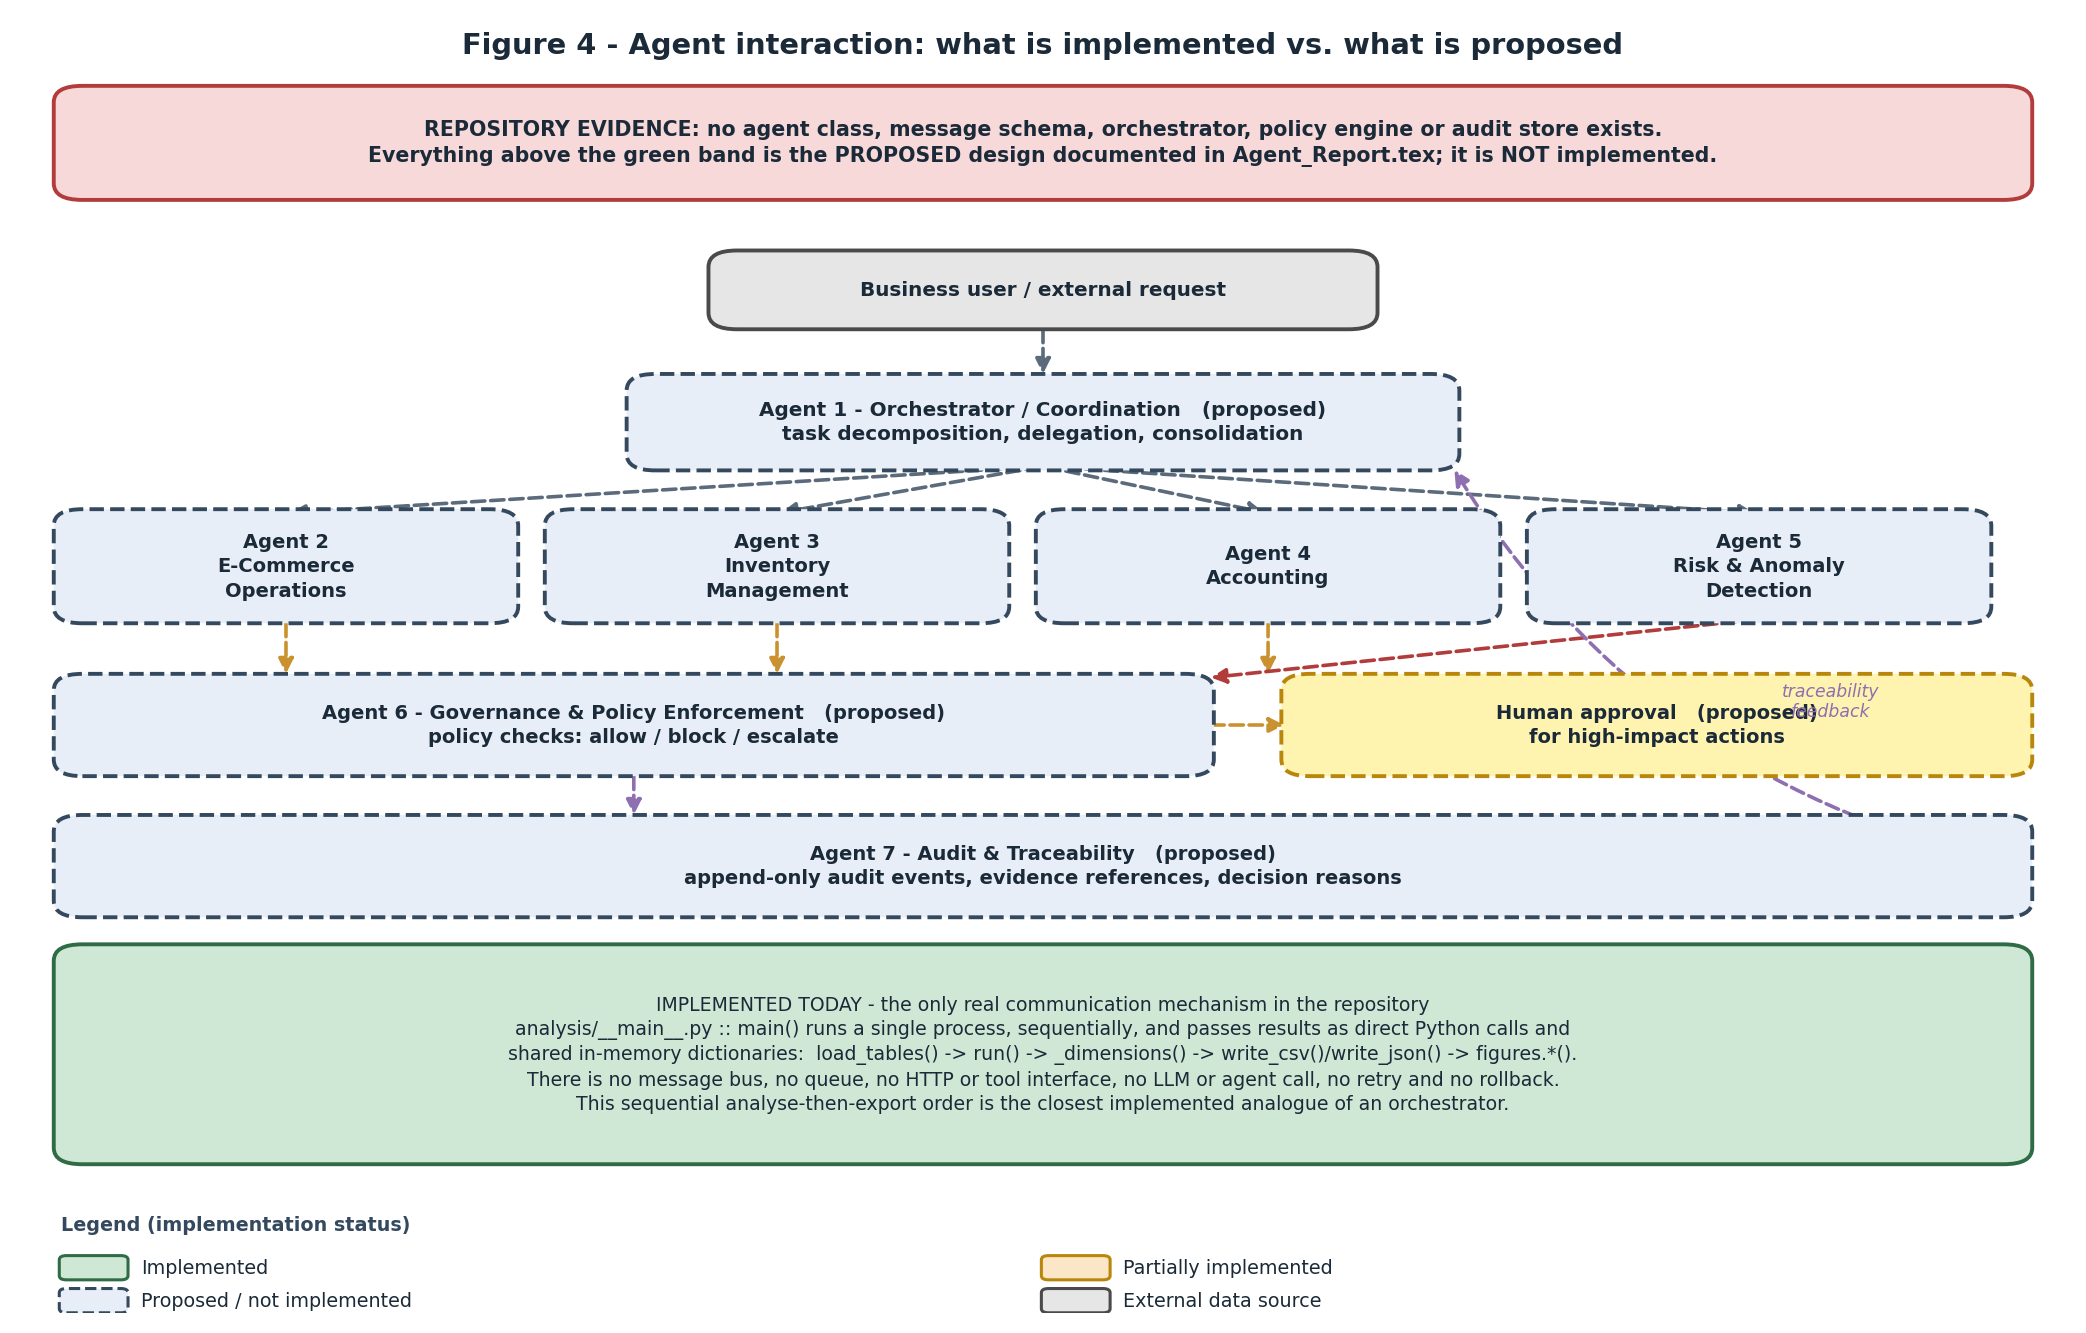
\includegraphics[width=\textwidth]{fig_agent_interaction.png}
\caption{Agent interaction. Everything above the green band is the proposed design; the green band is the only implemented communication mechanism, namely direct Python calls in a single sequential process.}
\label{fig:agents}
\end{figure}

% ===========================================================================
\section{Data Pipeline and Dataset Integration}
\label{sec:pipeline}
% ===========================================================================
Figure~\ref{fig:pipeline} presents the pipeline as implemented. The reader is referred to the Dataset Report for dataset characteristics; only the code's operations are described here.

\begin{figure}[H]\centering
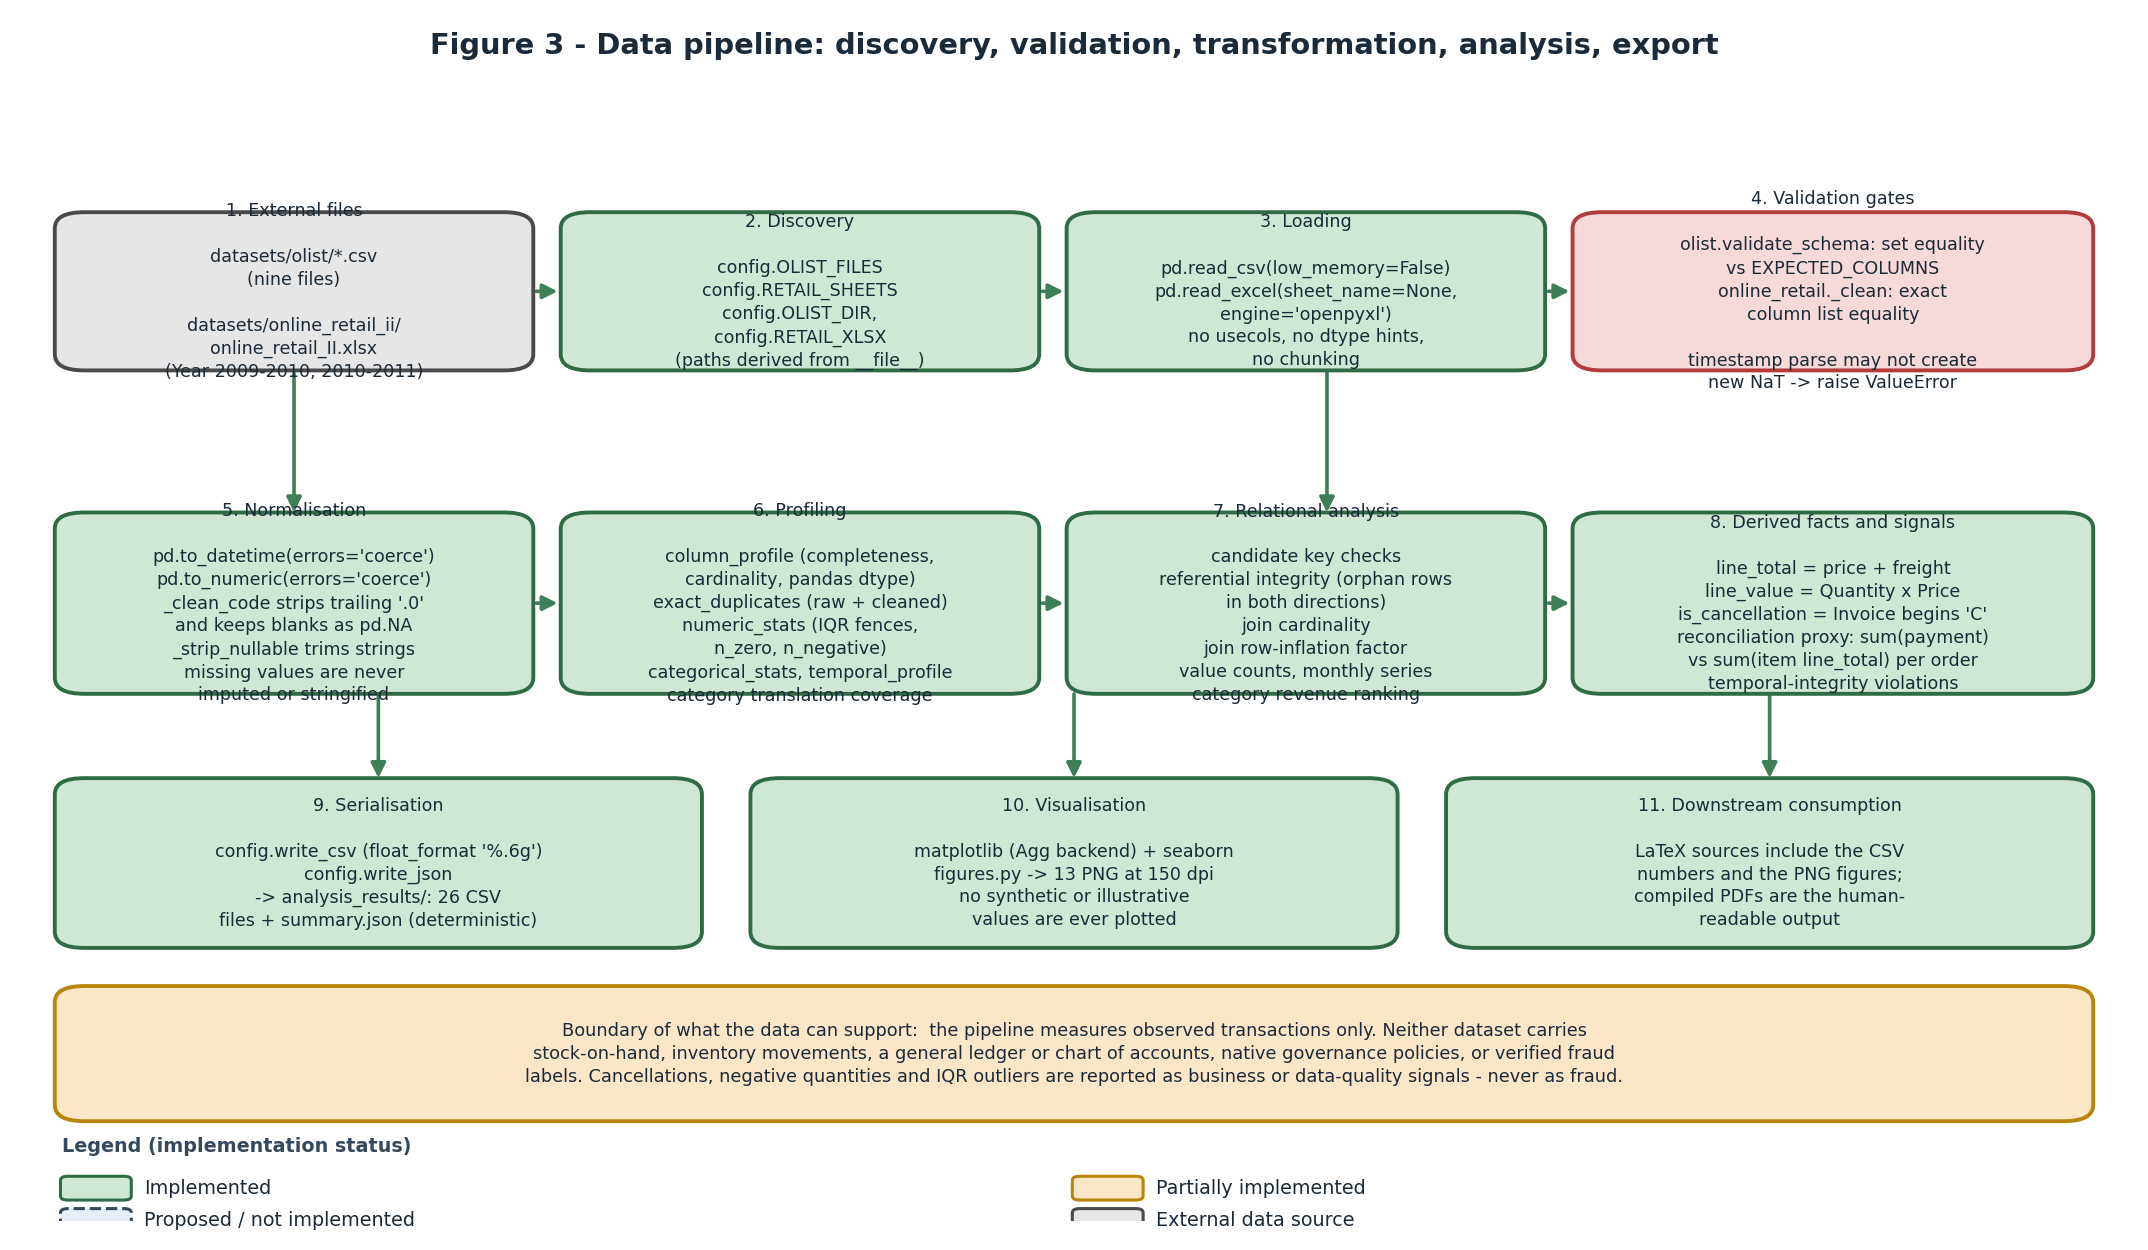
\includegraphics[width=\textwidth]{fig_data_pipeline.png}
\caption{The implemented data pipeline. Red marks the validation gates that abort the run on failure; amber marks the explicit statement of what the data cannot support.}
\label{fig:pipeline}
\end{figure}

\paragraph{Input discovery and loading.} \code{config.OLIST\_FILES} names the nine CSVs and \code{config.RETAIL\_SHEETS} names the two worksheets. Olist files are read with \code{pd.read\_csv(..., low\_memory=False)}; the workbook is read with \code{pd.read\_excel(..., sheet\_name=None, engine="openpyxl")}, which loads both sheets into memory. No \code{usecols}, \code{dtype}, chunk size or \code{parse\_dates} argument is supplied.

\paragraph{Formats and paths.} CSV with a UTF-8 BOM in the case of the inspector (opened with \code{encoding="utf-8-sig"}) and XLSX for the workbook. Paths are derived from \code{\_\_file\_\_}, so the package works from any working directory as long as it is invoked as a module from \code{reports/dataset\_report}.

\paragraph{Column selection and type conversion.} No columns are dropped. In Olist, only the columns listed in \code{DATE\_COLUMNS} are converted (to \code{datetime64}), protected by the non-regression gate. In the workbook, \code{\_clean} converts \code{InvoiceDate}, \code{Quantity}, \code{Price} and \code{Customer ID} with \code{errors="coerce"} and normalises the code and text columns.

\paragraph{Missing-value handling.} This is a deliberate design point consistent with established data-quality practice \cite{batini2009}: missing values are preserved, never imputed and never stringified. \code{\_clean\_code} maps blanks to \code{pd.NA}; \code{\_strip\_nullable} restores real missingness after a string operation; \code{value\_counts\_table} reports an explicit \code{<missing>} category; \code{column\_profile} reports \code{n\_missing} and \code{missing\_pct}. Four dedicated tests assert these behaviours.

\paragraph{Duplicate detection.} \code{exact\_duplicates()} counts exact duplicate rows; \code{olist.load\_tables()} separately records raw duplicates before parsing so that ``original-data duplicates'' and ``parsed duplicates'' remain distinguishable; the workbook reports duplicates both raw and after cleaning, plus repeated line keys.

\paragraph{Identifier validation.} \code{key\_check()} is applied to eleven candidate keys (single and composite, including \code{order\_id+order\_item\_id} and \code{order\_id+payment\_sequential}). \code{referential\_integrity()} checks six foreign-key relationships in both directions, reporting orphan rows and orphan percentages.

\paragraph{Transformations and joins.} Two derived fields are created: \code{line\_total = price + freight} for Olist order items and \code{line\_value = Quantity * Price} for the workbook. Joins are measured rather than materialised for analysis: \code{\_join\_expansion()} performs each candidate inner join only to record resulting row counts and an inflation factor, and \code{join\_cardinality} characterises each relationship.

\paragraph{Feature engineering.} Only the two derived value fields plus the cancellation flag and period columns (\code{month}) are engineered. No lag, rolling-window, frequency or basket features are produced.

\paragraph{Output generation.} Twenty-six CSV files and one JSON summary, plus thirteen PNGs. The summary embeds the \code{facts} dictionaries for both datasets and the list of figure paths.

\paragraph{Operations performed by code versus recommendations.} Everything listed above is executed by code. Two categories are \emph{not} executed and appear only as recommendations in the sibling reports: (i) canonical-event mapping and source adapters, and (ii) any inventory-position or ledger reconstruction. The code correctly refuses to assume information the data does not contain --- no stock levels, no ledger entries, no fraud labels.

\paragraph{A verified cross-tool inconsistency.} The two independent readers disagree about the size of one table. The pandas-based loader reports 99{,}224 rows for \code{olist\_order\_reviews\_dataset.csv}; the standard-library inspector reports 99{,}250. The cause was isolated: \code{csv.Sniffer().sniff(...)} infers a dialect with \code{doublequote=False}, so rows containing escaped quotes are split and embedded newlines produce 26 phantom records. The pandas count is the correct one (a plain \code{csv.DictReader} with the default dialect also yields 99{,}224). The incorrect figure appears in the inspector artifacts and in \code{main.tex}, and the resulting Olist total (1{,}550{,}948) differs from the Dataset Report total (1{,}550{,}922). This is reported as a defect, with the fix listed in Section~\ref{sec:limits}.

% ===========================================================================
\section{Data Contracts and Schemas}
\label{sec:schemas}
% ===========================================================================
\paragraph{What exists: implicit contracts.} There are no typed schemas in the implementation. No Pydantic model, dataclass, \code{TypedDict} or JSON Schema is defined anywhere; \code{pydantic} is not imported. The contracts that do exist are structural constants and the shape of the returned dictionaries:
\begin{itemize}
\item \code{olist.EXPECTED\_COLUMNS} --- the expected column list for each of the nine Olist tables, used as an executable contract by \code{validate\_schema()}.
\item \code{olist.DATE\_COLUMNS} --- which columns are parsed as timestamps and which are therefore subject to the non-regression gate.
\item \code{online\_retail.EXPECTED\_COLS} --- the exact eight-column contract enforced by \code{\_clean()}.
\item \code{config.OLIST\_FILES}, \code{config.RETAIL\_SHEETS}, \code{config.OLIST\_TABLE\_ORDER} --- the input inventory and presentation order.
\item The \code{frames}/\code{facts} dictionaries --- the informal internal interface between \code{run()} functions, \code{\_\_main\_\_} and \code{figures}. Their keys are implicit: \code{frames} holds named \texttt{DataFrame}s (for example \code{schema\_validation}, \code{column\_profile}, \code{reconciliation\_proxy} facts) and \code{facts} holds nested dictionaries. Because they are untyped, a typo or a renamed key would fail only at run time.
\item The output contract is likewise implicit: the column sets of the CSV artifacts exist only as the code that writes them. No schema file or test asserts them.
\end{itemize}

\paragraph{What does not exist: agent-facing contracts.} There is no request schema, no response schema, no task or workflow-state schema, no anomaly-record schema, no governance-decision schema and no audit-event schema. These are \textbf{proposed} in the sibling reports --- a data-contract section and an audit-event schema in the Agent Report, and an audit-event schema plus a canonical-event discussion in the Dataset Report --- and are not implemented. They are named here only to prevent any implication that they exist in code.

% ===========================================================================
\section{Agent Communication and Workflow Orchestration}
\label{sec:comms}
% ===========================================================================
\paragraph{Mechanism actually used.} The only communication mechanism is a direct synchronous Python function call, with results passed as plain dictionaries of \texttt{DataFrame}s in the calling process's memory. Read from \code{main()}, the control flow is:

\begin{verbatim}
config.ensure_dirs()
olist_tables, olist_raw_dups = olist.load_tables()
ol            = olist.run(olist_tables, olist_raw_dups)
retail_sheets = online_retail.load_sheets()
rt            = online_retail.run(retail_sheets)
dims, ol_dim, rt_dim = _dimensions(olist_tables, retail_sheets)
# 26 x config.write_csv(...) ; figures.*(...) ; config.write_json(...)
\end{verbatim}

A small number of minor side-channels exist and are worth recording: \code{olist.run()} stores private frames under keys prefixed with an underscore (\code{results["\_items"]}, \code{results["\_orders"]}, \code{results["\_cleaned"]}, \code{results["\_combined"]}) so that \code{figures} can reuse already-parsed data, and \code{online\_retail.run()} similarly exposes \code{\_cleaned} and \code{\_combined}. This is shared in-memory state, not messaging.

\paragraph{Mechanisms not used.} No message broker or queue, no HTTP endpoint, no RPC, no graph-based workflow engine, no LLM tool calling, no event bus and no persistence layer. The \code{PATH}-B inspector is an entirely independent program: it shares no code with the analysis package and reads the raw files again.

\paragraph{Retries, error propagation and conflicting results.} There is no retry logic, no timeout, no compensation and no dependency resolution. Error propagation is Python's default: the two validation gates raise \code{ValueError} with a message naming the file and column, and the process aborts. Because there is exactly one result per metric, there is no concept of conflicting results to reconcile. Any inter-agent messaging, retry or conflict-resolution design lives in the Agent Report and is explicitly proposed.

% ===========================================================================
\section{Governance, Security and Audit Implementation}
\label{sec:governance}
% ===========================================================================
Figure~\ref{fig:gov} separates the controls that the code actually enforces from those that exist only as documentation. Table~\ref{tab:controls} then attributes each control to a file or records its absence. The external reference points for the controls a governed AI system is normally expected to provide are the NIST AI Risk Management Framework \cite{nistAirmf2023,nistAi6001} and ISO/IEC 42001 \cite{iso42001}; this section measures the repository against that expectation.

\begin{figure}[H]\centering
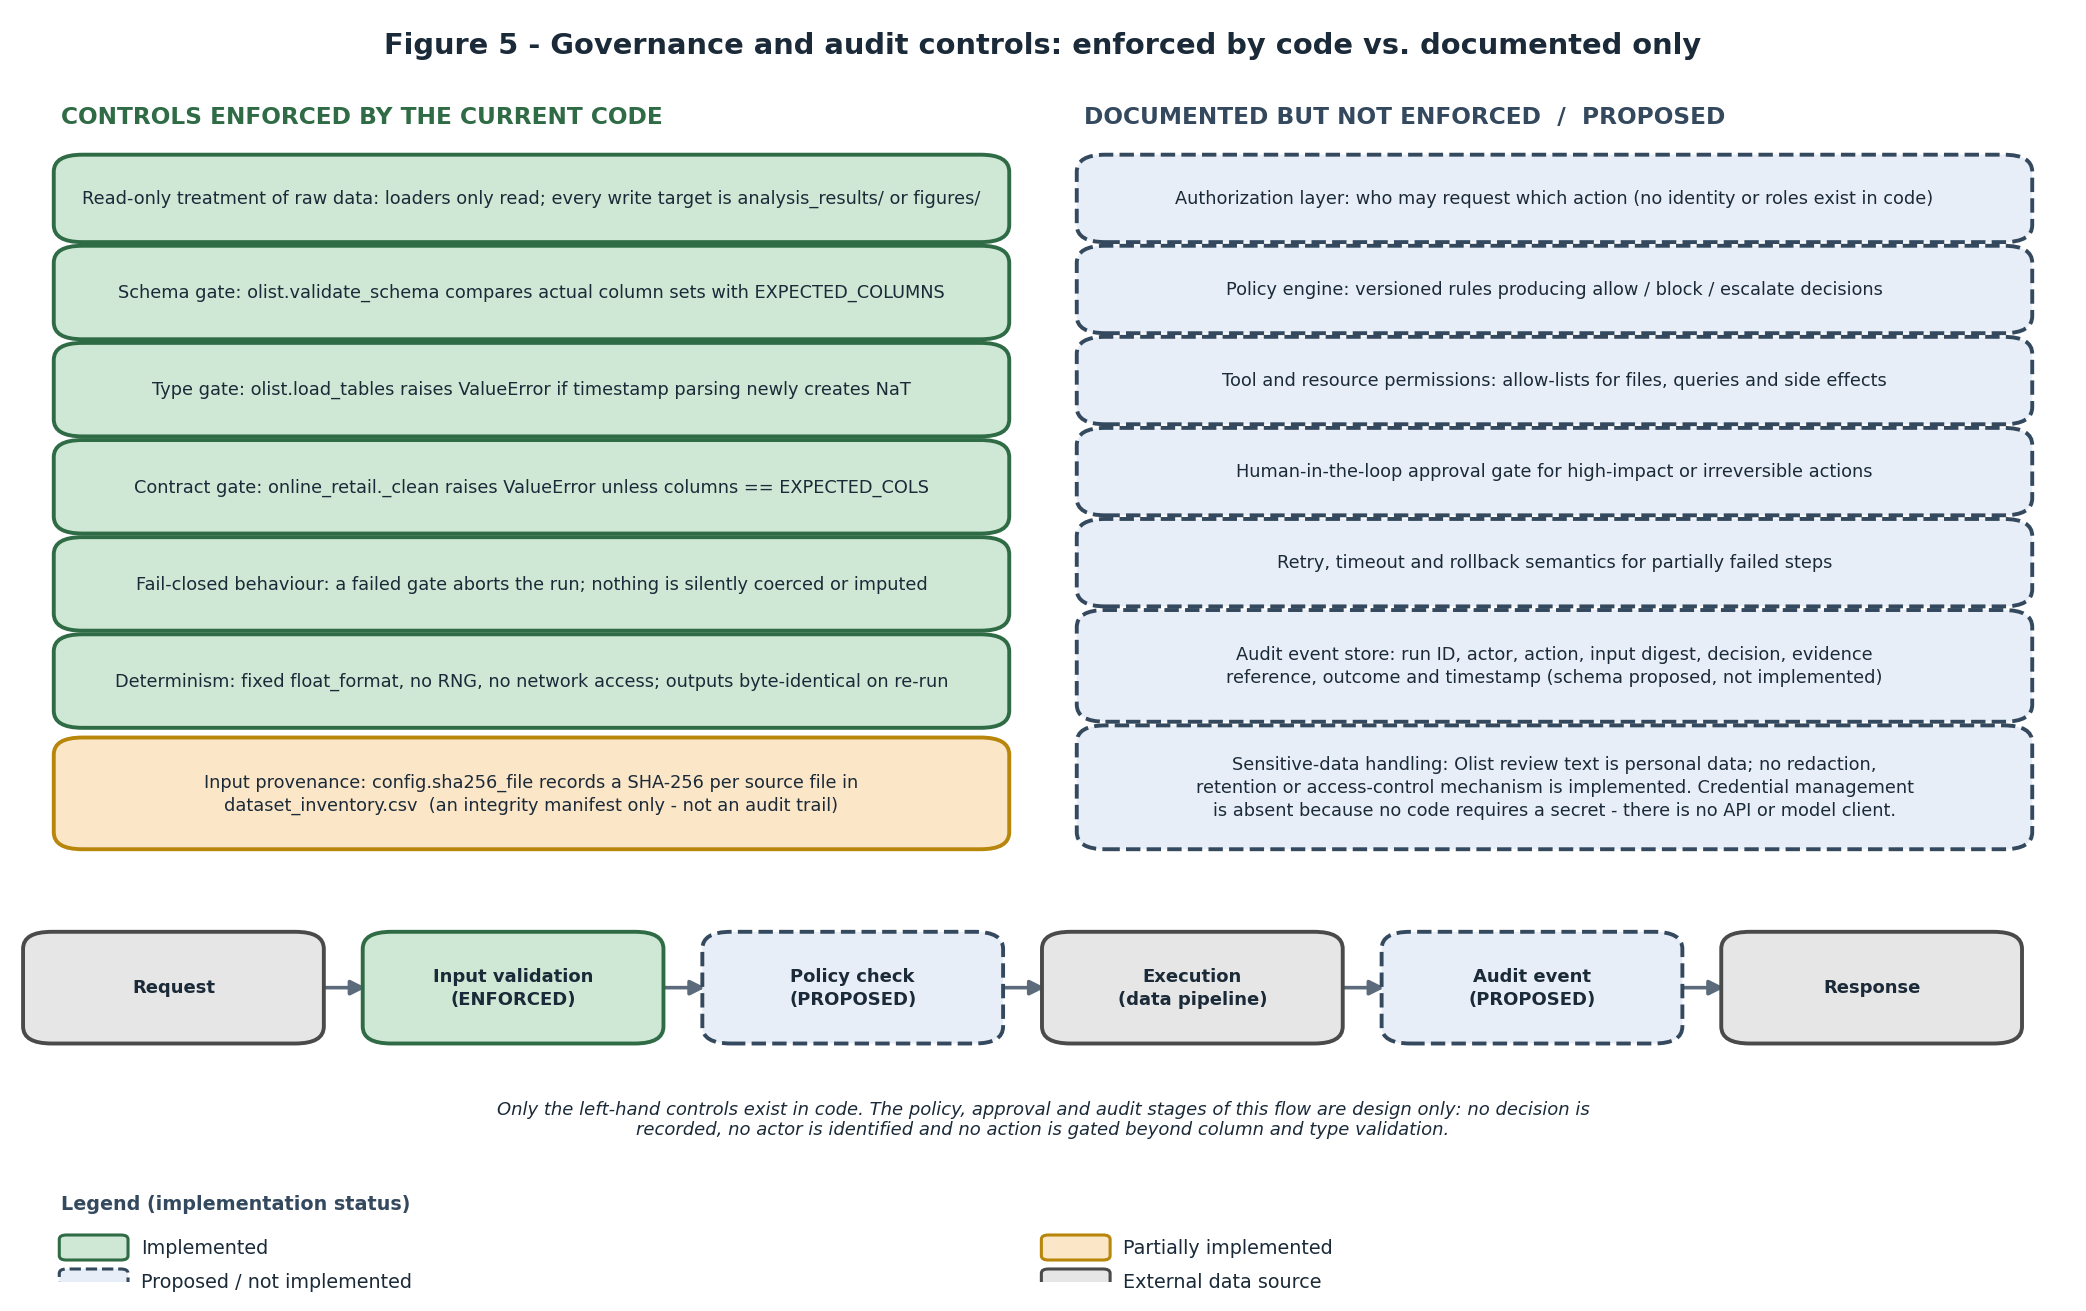
\includegraphics[width=\textwidth]{fig_governance_audit.png}
\caption{Governance and audit controls. The left column is enforced by code; the right column, and the middle of the flow strip, are design only.}
\label{fig:gov}
\end{figure}

\begin{table}[H]
\centering
\small
\begin{tabularx}{\textwidth}{L{3.6cm}L{3.4cm}X}
\toprule
\textbf{Control} & \textbf{Classification} & \textbf{Implementing file, or reason for absence} \\
\midrule
Raw-data immutability (by usage) & Enforced by software & \code{olist.load\_tables}, \code{online\_retail.load\_sheets}, \code{inspect\_datasets.xlsx\_rows} only read; every writer targets \code{analysis\_results/} or \code{figures/} \\
Input schema validation & Enforced by software & \code{olist.validate\_schema}; \code{online\_retail.\_clean} \\
Timestamp non-regression gate & Enforced by software & \code{olist.load\_tables} raises \code{ValueError} \\
Fail-closed abort on invalid structure & Enforced by software & the two \code{raise} statements; no silent coercion of key columns \\
Input provenance (integrity manifest) & Partially implemented & \code{config.sha256\_file} via \code{compare.dataset\_inventory}; digest only, no event, no timestamp, no actor \\
Deterministic, network-free execution & Enforced by software & \code{config.write\_csv} fixed \code{float\_format}; no network or random calls; verified byte-identical re-run \\
Authorization / access control & Not enforced & no identity, role or permission concept exists in any file \\
Policy evaluation (allow/block/escalate) & Documented but not enforced & described in the Agent Report; no policy data, rule file or engine in the repository \\
Tool / resource permissions & Documented but not enforced & no tool layer exists \\
Human-in-the-loop approval & Documented but not enforced & described in the Agent Report; no approval object or gate in code \\
Retry / rollback / timeout & Proposed & no retry, timeout or transaction semantics anywhere \\
Audit-event generation and store & Documented but not enforced & no event log, run ID, actor or decision record; \code{logging} is never imported \\
Sensitive-data handling & Documented but not enforced & Olist review text is personal data under regimes such as the GDPR \cite{gdpr2016}; no redaction, retention or access control is implemented \\
Credential management & Not applicable / absent & no API client, model provider or database connection exists, so no secret is required or stored \\
\bottomrule
\end{tabularx}
\caption{Every governance-relevant control found, classified as (1) enforced by the software, (2) documented but not enforced, or (3) proposed/absent. Applying the standard of Section~12 of the task, only the first five rows are technically enforced.}
\label{tab:controls}
\end{table}

% ===========================================================================
\section{Testing and Code Quality}
\label{sec:testing}
% ===========================================================================
\begin{figure}[H]\centering
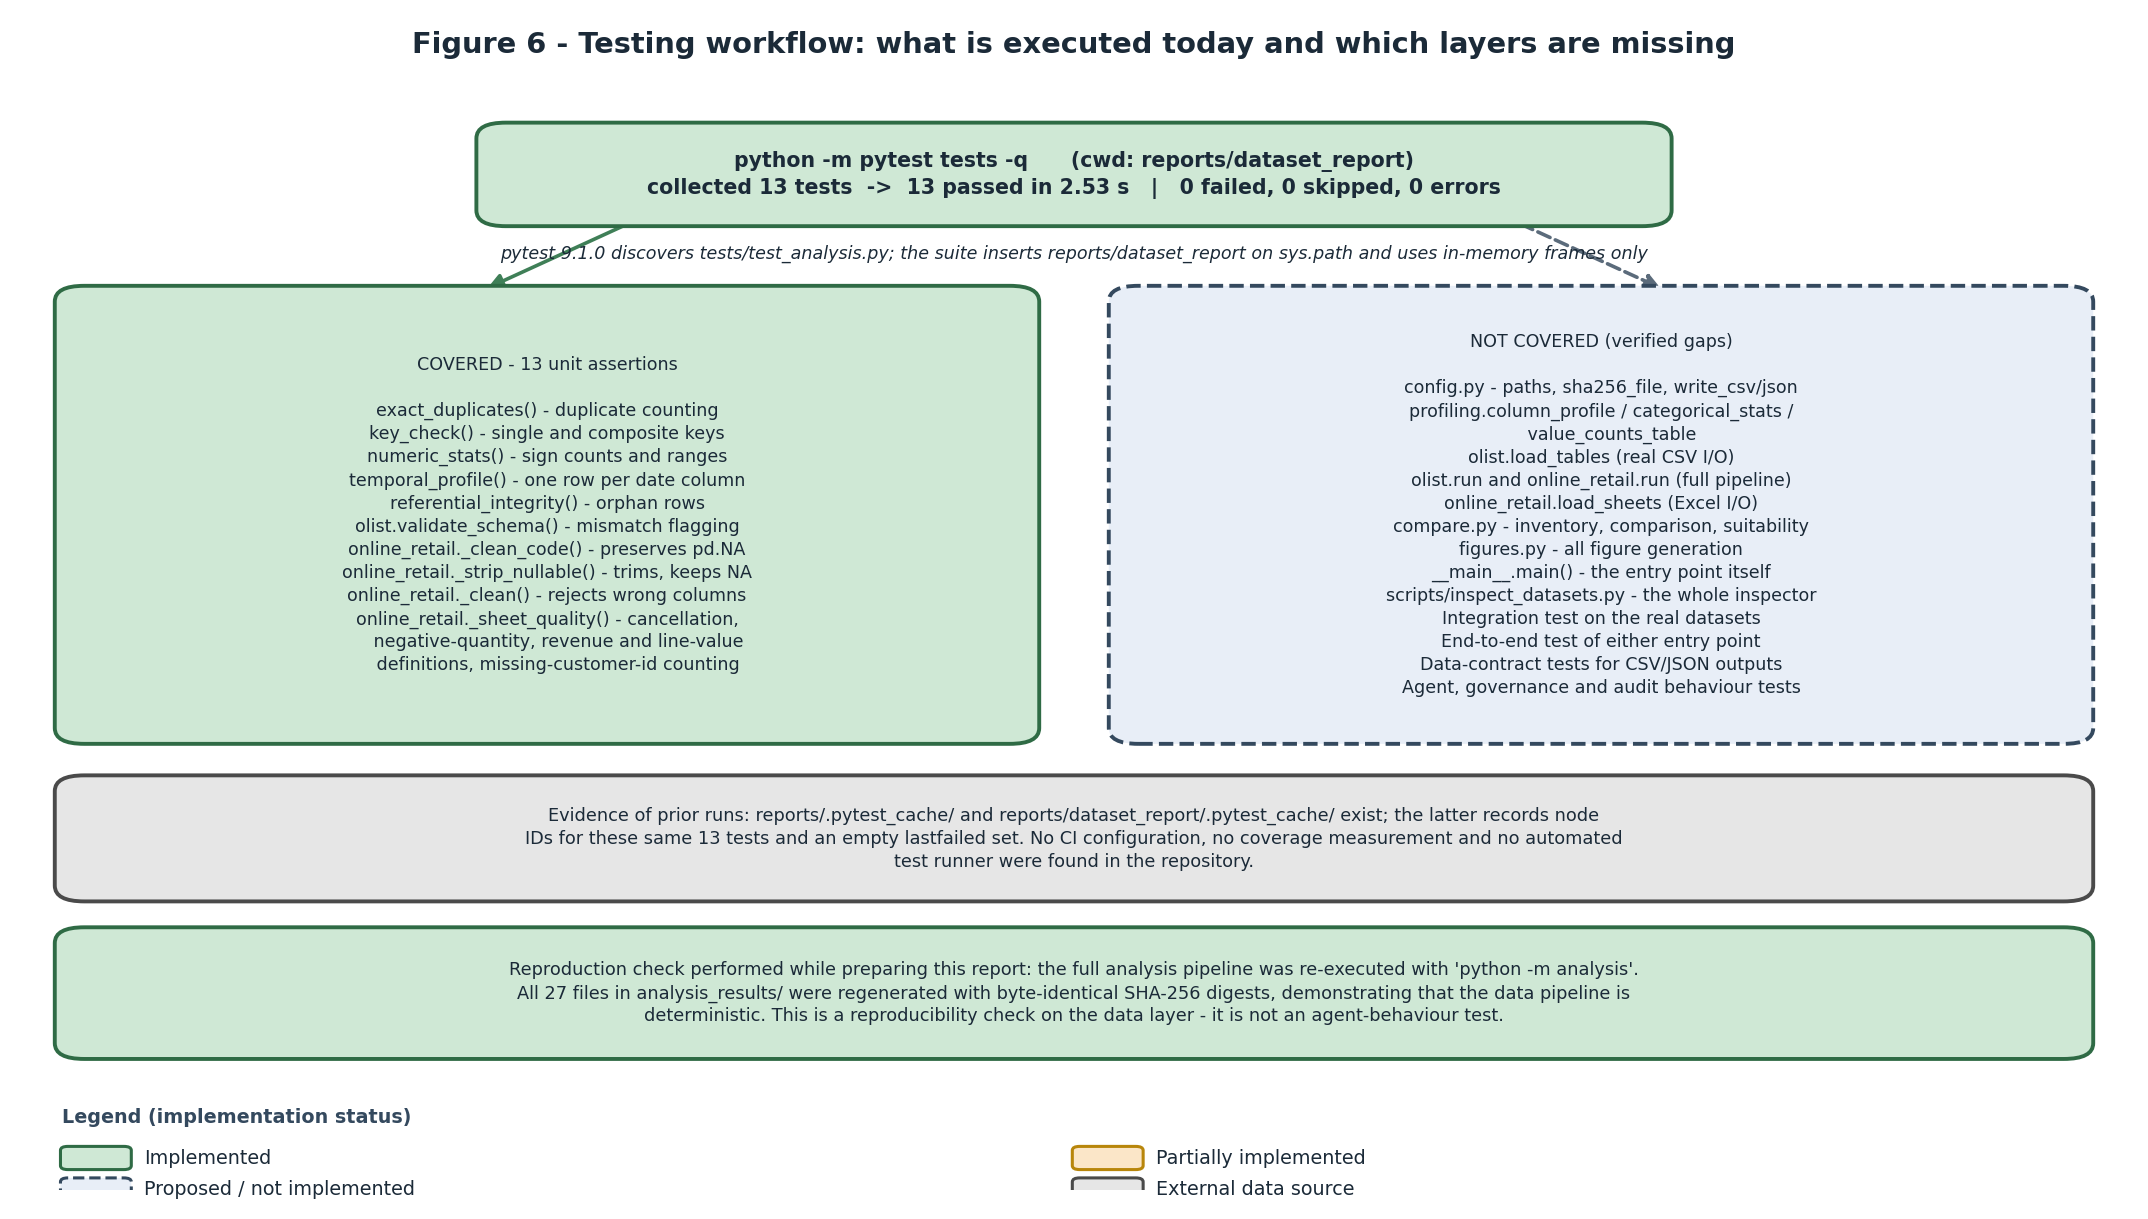
\includegraphics[width=\textwidth]{fig_testing_workflow.png}
\caption{Test coverage as measured. The left column is covered by the existing thirteen assertions; the right column is verified to be uncovered.}
\label{fig:testing}
\end{figure}

\paragraph{Framework and layout.} pytest 9.1.0. A single test module, \code{reports/dataset\_report/tests/test\_analysis.py} (177 lines, fourteen functions of which thirteen are tests), with no \code{conftest.py}, no \code{pytest.ini} and no \code{tox.ini}. The module inserts \code{Path(\_\_file\_\_).resolve().parents[1]} on \code{sys.path} so that \code{analysis} is importable, which is a workaround for the absence of an installed package.

\paragraph{Command executed and observed result.} The following command was run for this report, from \code{reports/dataset\_report}:
\begin{verbatim}
python -m pytest tests -q
.........                                                       [100%]
13 passed in 1.49s
\end{verbatim}
All thirteen tests passed; there were no failures, errors, skips or xfails. The tests use only small in-memory frames and never read the raw datasets, so they are fast and safe.

\paragraph{What the tests actually assert.} Missing-value preservation (\code{\_clean\_code}, \code{\_strip\_nullable}); exact-duplicate counting; composite-key uniqueness and duplicate detection; referential-integrity orphan counting in both directions; sign counts and ranges in \code{numeric\_stats}; one-row-per-column behaviour of \code{temporal\_profile}; cancellation detection and negative-quantity definitions; revenue and line-value definitions; missing-customer-identifier counting; Olist schema-mismatch flagging; and rejection of wrong columns by \code{\_clean}.

\paragraph{Reproducibility check performed.} The full pipeline was re-executed with \code{python -m analysis}. All 27 files in \code{analysis\_results/} were regenerated and every one was byte-identical (SHA-256) to the pre-existing artifact. This is a strong, verifiable statement about the data layer: the pipeline is deterministic. It says nothing about agent behaviour, because there is none.

\paragraph{Test layers that are absent.} There are no integration tests (nothing exercises \code{run()}, \code{load\_tables()}, \code{load\_sheets()} or the real files end to end), no end-to-end tests of either entry point, no data-contract tests for the CSV/JSON outputs, no test of \code{config}, \code{compare} or \code{figures}, and no tests for agents, governance or audit. Figure~\ref{fig:testing} lists these verified gaps.

\paragraph{Coverage gaps and recommended tests.} The most valuable additions, in order, are: (1) an integration test that runs each path on a small fixture directory and asserts output file names, column sets and key invariants; (2) contract tests asserting the column schema of every CSV artifact; (3) tests for \code{olist.load\_tables}'s failure behaviour on a deliberately corrupt timestamp column; (4) a regression test capturing the review-table row count (99{,}224) so that the inspector defect cannot recur silently; (5) tests for \code{compare} and \code{figures} smoke-import; and (6) once agents exist, unit tests for policy decisions and audit-event emission.

\paragraph{Tooling and code-quality observations.} There is no linter, formatter, type checker, coverage measurement or CI configuration. Evidence of prior pytest runs exists in \code{reports/.pytest\_cache/} and \code{reports/dataset\_report/.pytest\_cache/}; the latter records node IDs for the same thirteen tests and an empty \code{lastfailed} set, consistent with an all-passing suite. One vestigial assertion exists in the schema test (\code{assert good is not None}) and one dead statement in the inspector (line~99).

% ===========================================================================
\section{Execution and Reproducibility Guide}
\label{sec:exec}
% ===========================================================================
Every command below was executed during preparation of this report unless explicitly marked otherwise.

\paragraph{1. Prerequisites.} Python 3.10 (the verified interpreter is 3.10.11). A \LaTeX{} distribution (MiKTeX 24.1 was verified) is needed only to rebuild the reports.

\paragraph{2. Environment setup.} No virtual environment is configured in the repository. Create one if desired; no environment variables are read by any script (verified: \code{os.environ} is not used except for an implicit default in \code{inspect\_datasets.py}'s argument defaults).

\paragraph{3. Dependency installation.} \textbf{No dependency manifest exists}, so installation is inferred from imports and observed versions and is therefore partly \emph{unverified}. The versions below are those observed in the working environment:
\begin{verbatim}
python -m pip install pandas==2.3.3 numpy==1.26.4 matplotlib==3.10.7 \
    seaborn==0.13.2 openpyxl==3.1.5 pytest==9.1.0
\end{verbatim}
The inspector path requires \emph{no} third-party package.

\paragraph{4. Configuration setup.} None required. Paths are derived from the file locations; there is no configuration file, no secret and no environment variable to set.

\paragraph{5. Dataset placement.} The raw data must remain at \code{datasets/olist/*.csv} (nine files) and \code{datasets/online\_retail\_ii/online\_retail\_II.xlsx}. The analysis package computes \code{REPO\_ROOT} as the parent of \code{reports/}, so moving the datasets breaks the Olist loader and the workbook loader. The inspector accepts \code{--root} and \code{--output} and is therefore relocatable.

\paragraph{6. Execution commands.} Verified:
\begin{verbatim}
# analysis package (writes analysis_results/ and figures/)
python -m analysis            # run from reports/dataset_report

# independent inspector (stdlib only), run from the repository root
python reports/dataset_selection_table/scripts/inspect_datasets.py

# regenerate the diagrams of this report
python figures/make_figures.py   # from reports/code_report
\end{verbatim}
The workbook read is the slow step; the run prints a warning-free progress line and takes roughly one minute on the inspected machine.

\paragraph{7. Test commands.} Verified: \code{python -m pytest tests -q} from \code{reports/dataset\_report} (\code{13 passed}).

\paragraph{8. Output locations.} \code{reports/dataset\_report/analysis\_results/} (26 CSV + \code{summary.json}), \code{reports/dataset\_report/figures/} (13 PNG), \code{reports/dataset\_selection\_table/} (five CSV + \code{inspection\_summary.json}), and \code{reports/code\_report/figures/} (six PNG).

\paragraph{9. Troubleshooting.} \code{ModuleNotFoundError: analysis} means the command was run outside \code{reports/dataset\_report}; use the quoted working directory. \code{ValueError: ...: N values failed timestamp parsing} means an input file was modified or corrupted, and is the intended fail-closed behaviour. \code{ValueError: sheet '...' columns ... != expected ...} means the workbook structure changed. \code{ImportError: Missing optional dependency 'openpyxl'} means openpyxl is not installed. If a PDF is to be rebuilt, run the four-pass \code{pdflatex}/\code{bibtex}/\code{pdflatex}/\code{pdflatex} sequence; a path containing a space such as \code{reports/Agents reports} must be quoted on Windows.

% ===========================================================================
\section{Outputs and Evaluation}
\label{sec:outputs}
% ===========================================================================
\subsection{Artifacts produced by the code}
Table~\ref{tab:outputs} lists the artifacts. No output is a performance measurement.

\begin{table}[H]
\centering
\small
\begin{tabularx}{\textwidth}{L{5.0cm}L{1.6cm}L{4.2cm}X}
\toprule
\textbf{Artifact} & \textbf{Format} & \textbf{Generating module} & \textbf{Meaning and intended use} \\
\midrule
\code{analysis\_results/table\_dimensions.csv} & CSV & \code{\_\_main\_\_.\_dimensions} & Rows and columns per table/sheet \\
\code{.../olist\_schema\_validation.csv} & CSV & \code{olist.validate\_schema} & Schema conformance per Olist table \\
\code{.../olist\_column\_profile.csv} & CSV & \code{profiling.column\_profile} & Completeness and cardinality per column \\
\code{.../olist\_duplicate\_rows.csv} & CSV & \code{profiling.exact\_duplicates} & Raw and parsed duplicate counts \\
\code{.../olist\_numeric\_stats.csv} & CSV & \code{profiling.numeric\_stats} & Distribution, quartiles, IQR outlier counts \\
\code{.../olist\_categorical\_stats.csv} & CSV & \code{profiling.\allowbreak categorical\_stats} & Top categories and cardinality \\
\code{.../olist\_temporal\_profile.csv} & CSV & \code{profiling.temporal\_profile} & Per-column timestamp ranges and spans \\
\code{.../olist\_primary\_key\_checks.csv} & CSV & \code{profiling.key\_check} & Candidate keys and duplicate excess \\
\code{.../olist\_referential\_integrity.csv} & CSV & \code{olist.referential\_integrity} & Orphan rows per foreign key, both directions \\
\code{.../olist\_join\_cardinality.csv} & CSV & \code{olist.run} & Relationship cardinality and child counts \\
\code{.../olist\_join\_expansion.csv} & CSV & \code{olist.\_join\_expansion} & Inner-join row inflation factors \\
\code{.../olist\_value\_counts.csv} & CSV & \code{profiling.value\_counts\_table} & Status, payment type, review score, state, category \\
\code{.../olist\_category\_revenue.csv} & CSV & \code{olist.run} & Top categories by item value \\
\code{.../olist\_monthly\_orders.csv} & CSV & \code{olist.run} & Order volume by purchase month \\
\code{.../retail\_*.csv} (nine files) & CSV & \code{online\_retail.run} & Workbook profiles, quality metrics, business signals \\
\code{.../dataset\_inventory.csv} & CSV & \code{compare.dataset\_inventory} & File sizes and SHA-256 digests \\
\code{.../dataset\_comparison.csv} & CSV & \code{compare.dataset\_comparison} & Curated comparison (mixed measured and qualitative) \\
\code{.../agent\_suitability.csv} & CSV & \code{compare.agent\_suitability} & Curated per-agent suitability (qualitative) \\
\code{.../summary.json} & JSON & \code{\_\_main\_\_.main} & Aggregated facts for both datasets \\
\code{figures/fig\_*.png} (13 files) & PNG & \code{figures} & Report figures computed from the real data \\
\code{dataset\_selection\_table/*.csv} & CSV & \code{inspect\_datasets.main} & Independent inventory, quality, key and suitability tables \\
\code{dataset\_selection\_table/\linebreak inspection\_summary.json} & JSON & \code{inspect\_datasets.main} & Machine-readable inventory and relationship checks \\
\bottomrule
\end{tabularx}
\caption{Artifacts generated by the code. \code{analysis\_results} contains 26 CSV files plus \code{summary.json}; the file list above groups the nine retail CSVs.}
\label{tab:outputs}
\end{table}

\subsection{Evaluation status and proposed plan}
\textbf{No evaluation of the multi-agent system has been performed, because no multi-agent system exists.} There are no experiment logs, no baselines, no metrics and no results tables for agent behaviour in the repository. The Dataset Report and the Agent Report contain \emph{proposed} evaluation protocols; those remain proposals. This Code Report therefore proposes a code-oriented evaluation plan consistent with what will actually be built:
\begin{itemize}
\item \textbf{Ingestion and validation layer.} Metrics: schema-gate pass rate on a frozen input corpus; determinism rate (currently 100\% over 27 artifacts); median runtime; memory peak. Baselines: the current pipeline.
\item \textbf{Orchestration.} Metrics: workflow completion rate, dependency-violation count, retry count, end-to-end latency on replayed orders. Baseline: the current manual sequence.
\item \textbf{Governance.} Metrics: policy-decision accuracy against a hand-labelled rule set, false-block rate, and the fraction of high-impact actions routed to approval. Baseline: column/type validation only.
\item \textbf{Audit.} Metric: evidence-traceability rate --- the fraction of decisions for which every source record referenced can be resolved. Baseline: none (no event log exists).
\item \textbf{Reproducibility and limitations.} Every reported number must be regenerable by one documented command on a pinned environment; the absence of fraud labels means no detector accuracy will be reported.
\end{itemize}

% ===========================================================================
\section{Limitations and Technical Debt}
\label{sec:limits}
% ===========================================================================
Findings are separated into \emph{verified defects} (reproduced during this inspection) and \emph{risks}. Severity is an engineering judgement.

\begin{table}[H]
\centering
\footnotesize
\begin{tabularx}{\textwidth}{L{0.7cm}L{4.1cm}L{1.6cm}X}
\toprule
\textbf{ID} & \textbf{Finding} & \textbf{Type / severity} & \textbf{Evidence and recommended fix} \\
\midrule
D1 & \code{src/} is empty and the root \code{README.md} is 0 bytes & Verified / high & Directory and file listing; \code{(Get-Item README.md).Length = 0}. Fix: remove the placeholder or populate it as the real package root and installation entry point. \\
D2 & Reviewer/inspector over-counts the Olist review table by 26 rows & Verified defect / high & \code{csv.Sniffer} yields \code{doublequote=False}, producing 99{,}250 rows versus the correct 99{,}224 (pandas and default \code{csv.DictReader} agree). The error propagates to the inspector's \code{dataset\_inventory.csv} and \code{inspection\_summary.json}, and \code{main.tex} displays the inflated 99{,}250. Fix: pass an explicit dialect with \code{doublequote=True}, or drop \code{Sniffer} in favour of a fixed dialect. \\
D3 & No dependency manifest & Verified / high & No \code{requirements.txt}, \code{pyproject.toml} or lock file. Fix: add a pinned \code{requirements.txt} (or \code{pyproject.toml}) with the versions in Table~\ref{tab:tech}. \\
D4 & No output validation or assertion on generated artifacts & Verified / medium & \code{main()} writes and prints; nothing checks schema or counts. Fix: add a post-write contract check. \\
D5 & No logging; progress via \code{print()} & Verified / medium & \code{logging} is never imported. Fix: adopt \code{logging} with a run identifier. \\
D6 & Analysis package has no CLI & Verified / low & No \code{argparse} in \code{analysis}; inputs are hard-coded lists. Fix: add \code{--olist-dir}, \code{--retail-xlsx}, \code{--out}, \code{--figures}. \\
D7 & Bare \code{except} clauses and dead code in the inspector & Verified / low--medium & Lines~50--54, 94--95, 107--129 swallow errors; line~99 builds an unused \code{Counter}. Fix: narrow exception types and delete the dead statement. \\
D8 & Fragile path derivation in the inspector & Verified / low & \code{ROOT = Path(\_\_file\_\_).resolve().parents[3]}. Fix: use \code{--root} or resolve upward until a marker file is found. \\
D9 & Curated text mixed with measured data in one artifact & Verified / medium & \code{compare.dataset\_comparison} and \code{agent\_suitability} contain hand-written strings; the docstring acknowledges this. Fix: separate measured and interpretive columns, or mark them explicitly. \\
D10 & Whole-dataset memory load & Verified / low & \code{read\_csv(low\_memory=False)} and \code{read\_excel(sheet\_name=None)} load both sheets and all tables at once. Fix: chunking or per-sheet streaming if the corpus grows. \\
D11 & Code and generated artifacts share one directory & Verified / low & \code{analysis/} sits beside \code{analysis\_results/} and \code{figures/}. Fix: move the package to \code{src/} and treat \code{reports/} as output only. \\
D12 & Test-module \code{sys.path} hack and vestigial assertion & Verified / low & \code{sys.path.insert} at test import; \code{assert good is not None}. Fix: install the package or add \code{conftest.py}; delete the no-op assertion. \\
R1 & No governance/audit primitives at all & Risk / high & Required before any agent can act under policy. Fix: implement the policy gate and the audit store first (roadmap phase~3). \\
R2 & No fraud labels, no stock data, no ledger & Risk / medium & Stated in both datasets and in \code{agent\_suitability}. Fix: keep claims scoped; treat outputs as anomaly candidates. \\
R3 & Two divergent readers of the same corpus & Risk / medium & \code{analysis} (pandas) and \code{inspect\_datasets} (stdlib) duplicate profiling logic and have already diverged (D2). Fix: keep one canonical implementation and derive the other as a thin adapter. \\
R4 & No CI or automated runner & Risk / medium & No workflow file. Fix: add a minimal CI job running the tests and a determinism check. \\
\bottomrule
\end{tabularx}
\caption{Prioritized findings. D2, D3, D4 and R1 have the highest immediate impact on correctness and on the roadmap.}
\label{tab:limits}
\end{table}

\paragraph{Note on integrity claims.} Because the code has no event log and no integrity primitive beyond the file digests, the project must not describe the current system as auditable, tamper-evident or compliant. Those properties are proposed, not present.

% ===========================================================================
\section{Development Roadmap}
\label{sec:roadmap}
% ===========================================================================
The phases are ordered so that nothing already implemented is rebuilt, and so that governance and audit exist before any agent is allowed to act. Effort estimates are engineering judgements, not commitments.

\begin{table}[H]
\centering
\small
\begin{tabularx}{\textwidth}{L{1.1cm}L{4.3cm}L{4.4cm}X}
\toprule
\textbf{Phase} & \textbf{Goal} & \textbf{Deliverable} & \textbf{Depends on} \\
\midrule
1 & Stabilise the data pipeline & Fix D2; add D4 output contracts; fix D7/D8 in the inspector; freeze a small fixture corpus & nothing \\
2 & Pin the environment and package the code & Add \code{requirements.txt} (D3); move the package to \code{src/} (D11, D1) with \code{pyproject.toml}; remove the test \code{sys.path} hack & phase~1 \\
3 & Implement the governance gate and the audit store first & Versioned policy rule set, allow/block/escalate decision, append-only event writer with run IDs and evidence references & phase~2 \\
4 & Define and freeze the typed data contracts & Pydantic or dataclass models for canonical events, agent requests/responses, decisions and audit events, each with tests & phase~2 \\
5 & Complete the orchestrator & Task object, deterministic planner, specialist dispatch, dependency resolution, failure propagation, result consolidation --- all routed through phase~3 gates & phases~3--4 \\
6 & Implement the specialist agents one at a time & Reuse the existing data layer directly: E-Commerce on \code{olist.run} outputs; Accounting on the reconciliation proxy; Risk on the IQR/negative-quantity signals; Inventory strictly as a demand-indicator agent with an explicit data-gap declaration & phase~5 \\
7 & Add integration and end-to-end tests & Fixture-based pipelines, contract tests, scenario tests for approval, rejection and audit traceability & phases~5--6 \\
8 & Establish reproducible evaluation & The metrics in Section~\ref{sec:outputs}, with baselines and a one-command harness & phase~7 \\
9 & Documentation and deployment readiness & Replace the empty README; document the contracts; add CI (R4); containerise if required & phases~2--8 \\
\bottomrule
\end{tabularx}
\caption{Prioritized roadmap. Phases~3 and~4 deliberately precede agent implementation: without a policy gate and an audit store, no agent action would be governable or traceable.}
\label{tab:roadmap}
\end{table}

% ===========================================================================
\section{Conclusion}
% ===========================================================================
\textbf{What has been implemented.} A reproducible dataset analysis, validation and reporting pipeline of 2{,}144 lines of Python across eleven files, comprising the package \code{reports/dataset\_report/analysis/} with seven modules and a \code{python -m analysis} entry point, an independent standard-library inspector, and two figure generators for the sibling reports. The pipeline reads both research datasets read-only, applies two fail-closed structural gates, profiles nine Olist tables and two workbook sheets, measures keys, referential integrity, joins, distributions, temporal and monetary properties, derives a payment-versus-item reconciliation proxy and several workbook business signals, and exports 26 CSV files, one JSON summary and thirteen figures.

\textbf{What currently works.} The pipeline and the inspector execute successfully; the thirteen unit tests pass (\code{13 passed in 1.49\,s}); the pipeline is deterministic, with all 27 regenerated artifacts byte-identical; and the code correctly refuses to invent stock levels, ledger entries, policies or fraud labels. The repository also contains three coherent \LaTeX{} reports.

\textbf{What has been tested.} Only the data layer, and only at helper level: thirteen assertions over missing-value handling, duplicate counting, key checks, referential integrity, sign counts, temporal profiling, cancellation and revenue definitions, and schema validation. There is no integration, end-to-end, contract, agent, governance or audit test.

\textbf{What remains incomplete.} Everything above the ingestion and analysis layer. The repository has zero classes, no orchestrator, no messaging, no typed contracts, no policy engine, no approval mechanism and no audit event store; \code{src/} is empty and the root README is empty. All seven agents are \emph{designed but not implemented}. Three defects were verified during this inspection, the most concrete being the inspector's 26-row over-count of the Olist review table caused by an incorrectly inferred CSV dialect.

\textbf{How the code supports the research objectives.} The pipeline is precisely the ingestion and validation layer that the proposed architecture requires: it establishes stable, tested, reproducible access to both datasets and produces trustworthy measured facts that the sibling reports reuse. It gives the project a credible foundation and a clear, verified statement of the distance to a functioning governed multi-agent system. The roadmap in Section~\ref{sec:roadmap} closes that distance in a disciplined order, with governance and audit implemented before any agent is permitted to act.

% ===========================================================================
% REFERENCES
% ===========================================================================
\section{References and Technical Documentation}
\label{sec:refs}
The bibliography below reuses the references already present in the sibling reports' \code{references.bib} files and adds official documentation for the libraries that the code actually imports. Every entry was checked at the time of writing: the eight software-documentation URLs, the two dataset landing pages and the dataset DOIs returned HTTP~200, and the Crossref metadata for the journal, conference and NIST entries was retrieved and matched by DOI. The ISO catalogue page for ISO/IEC 42001 is the canonical address but refuses automated requests, as do some publisher pages; these respond normally in a browser. No citation, author, year, DOI or URL has been invented.

\bibliographystyle{plain}
\bibliography{references}

% ===========================================================================
% APPENDIX
% ===========================================================================
\appendix
\section{Repository Inventory and Verification Log}
\label{app:log}

\subsection*{A.1 Code inventory}
Eleven Python files, 2{,}144 lines, 65 functions, 0 classes (Table~\ref{tab:inventory}). Seven analysis modules plus \code{\_\_init\_\_} and \code{\_\_main\_\_}; one test module; one inspector; one figure generator for the Agent Report. No dependency manifest, no CI configuration, no container definition, no environment-variable usage, no credential material.

\subsection*{A.2 Commands executed for this report}
\begin{itemize}
\item \code{python --version} $\rightarrow$ \code{Python 3.10.11}; \code{pip list} $\rightarrow$ the versions in Table~\ref{tab:tech}.
\item \code{pdflatex --version} $\rightarrow$ MiKTeX-pdfTeX 4.18 (MiKTeX 24.1); \code{bibtex --version} $\rightarrow$ MiKTeX-BibTeX 4.1.
\item \code{cd reports/dataset\_report; python -m pytest tests -q} $\rightarrow$ \code{13 passed in 1.49s}.
\item \code{cd reports/dataset\_report; python -m analysis} $\rightarrow$ completed; 26 CSV + \code{summary.json} + 13 PNG written; all 27 \code{analysis\_results} files byte-identical to the pre-existing artifacts (SHA-256).
\item \code{python reports/dataset\_selection\_table/scripts/inspect\_datasets.py --output <temp>} $\rightarrow$ inspected 10 data files (nine Olist CSVs, one workbook) and wrote its artifacts to a temporary directory, leaving the committed artifacts untouched.
\item \code{python reports/code\_report/figures/make\_figures.py} $\rightarrow$ six PNGs.
\end{itemize}

\subsection*{A.3 Defect reproduction (D2)}
\begin{verbatim}
csv.Sniffer().sniff(sample).doublequote      -> False
sum(1 for _ in csv.DictReader(open(reviews), dialect=sniffed))  -> 99250
sum(1 for _ in csv.DictReader(open(reviews)))                   -> 99224
len(pandas.read_csv(reviews, low_memory=False))                 -> 99224
\end{verbatim}
The 26-row discrepancy is therefore produced by dialect detection, not by the file.

\subsection*{A.4 Integrity of sibling reports}
\code{main.tex}/\code{main.pdf}, \code{dataset\_report.tex}/\allowbreak\code{dataset\_report.pdf} and \code{Agent\_Report.tex}/\allowbreak\code{Agent\_Report.pdf} were read but not modified while preparing this report. The only written locations are \code{reports/code\_report/} (this report and its figures) and the regenerated deterministic artifacts under \code{reports/dataset\_report/} and the temporary inspector output. No source file was altered.

\end{document}
